\documentclass{sig-alternate-05-2015}

\usepackage{graphicx} % for images
\graphicspath{ {./images/} }
\usepackage{algorithm}
\usepackage[noend]{algpseudocode}
\usepackage{multicol}
\usepackage[utf8]{inputenc}
\usepackage[dvipsnames]{xcolor}
\usepackage{pgfplots}
\usepackage{hyperref}
\usepackage{caption} % for subfigures
\usepackage{subcaption} % for subfigures
\usepackage{url} % for breaking long URLs

\newtheorem{lemma}{Lemma}

\newtheorem{defn}{Definition}[section]

\newcommand{\query}{SkNGeo}
\newcommand{\rrp}{RRP}
\newcommand{\rrpsocial}{RRP-Social}
\newcommand{\rrpspatial}{RRP-Spatial}

\begin{document}

\title{\LARGE \bf RangeReachPaths(TODO): Answering Social Proximity Queries with GeoSpatial Range Filters}

\numberofauthors{3} 
\author{
% 1st. author
\alignauthor
Nitin Pasumarthy\\
       \affaddr{Arizona State University}\\
       \affaddr{Tempe, AZ}\\
       \email{npasumar@asu.edu}
% 2nd. author
\alignauthor
Yuhan Sun\\
       \affaddr{Arizona State University}\\
       \affaddr{Tempe, AZ}\\
       \email{Yuhan.Sun.1@asu.edu}
% 3rd. author
\alignauthor
Mohamed Sarwat\\
       \affaddr{Arizona State University}\\
       \affaddr{Tempe, AZ}\\
       \email{msarwat@asu.edu}
}

\maketitle
\begin{abstract}
Social media has become an effective advertising tool due to its ever increasing usage and influence. And with rapid increase in the usage of mobile phones and wearables, social media data is being tied to spatial networks. We propose a new query in this geo-social domain called the social proximity with geospatial range predicate. We perform a joint search on both these domains which radically improves the performance compared to straight forward solutions. We then experimentally prove how our approach out performs existing baseline approaches by at least 3 times and also compare how each of our algorithms perform under various conditions on a real geo-social dataset.
\end{abstract}

\printccsdesc

\keywords{socio-spatial; graphs; closest vertices; top-k; landmarks}

\section{Introduction}
A social network is a graph of individuals and their interactions. It is a great resource to keep upto date what an individual's friends are upto. With the ever increasing use of web, social media is also used as an advertising tool. They are proved quite effective~\cite{F1969},~\cite{JP1987},~\cite{PM2001} to gain quick popularity by publicizing on popular social media sites like Facebook, MySpace, BlogSphere etc. than traditional advertising means. Their effectiveness is mainly due to high usage and size of users using it. Facebook for example has around 1.59 billion active users monthly~\footnote{http://www.statista.com/statistics/264810/number-of-monthly-active-facebook-users-worldwide/}. Another popular micro-blogging site called twitter has about 310 million monthly active users~\footnote{http://www.statista.com/statistics/282087/number-of-monthly-active-twitter-users/}. With such massive networks generating lot of data, everyone is constantly looking into ways of integrating the knowledge from them to make their systems more personal for their end users. Microsoft now ranks results, in its BING search, for a user using the search history from his/her social network~\cite{M2011}. There are also works on how probable a user performs an action given his/her friend committed the same action before~\cite{DJE2003}. The natural problem of social influence would be, `given a social network, how can we detect the players through which we can spread, or “diffuse”, the new technology in the most effective way`~\cite{EA2007}. Spread maximizing problem which try to find a minimal set S in a graph to gain maximum spread in a network is well studied in~\cite{MP2002}.

At the other end of the spectrum are the spatial networks. With the ever increasing number of wearables everyday like Jawbone, Fitbit, smart watches (pebble, apple watch) there is an abundance of data in this realm too. Importantly with the rapid increase in the number of mobile phone users, this data is already being tied to Social Network data and the two realms are coming together. Popular social network sites like Facebook have a number of features which prompt users to add spatial information like check-ins, traveling posts, geotagged photos etc.

\begin{figure}[t]
	\centering
	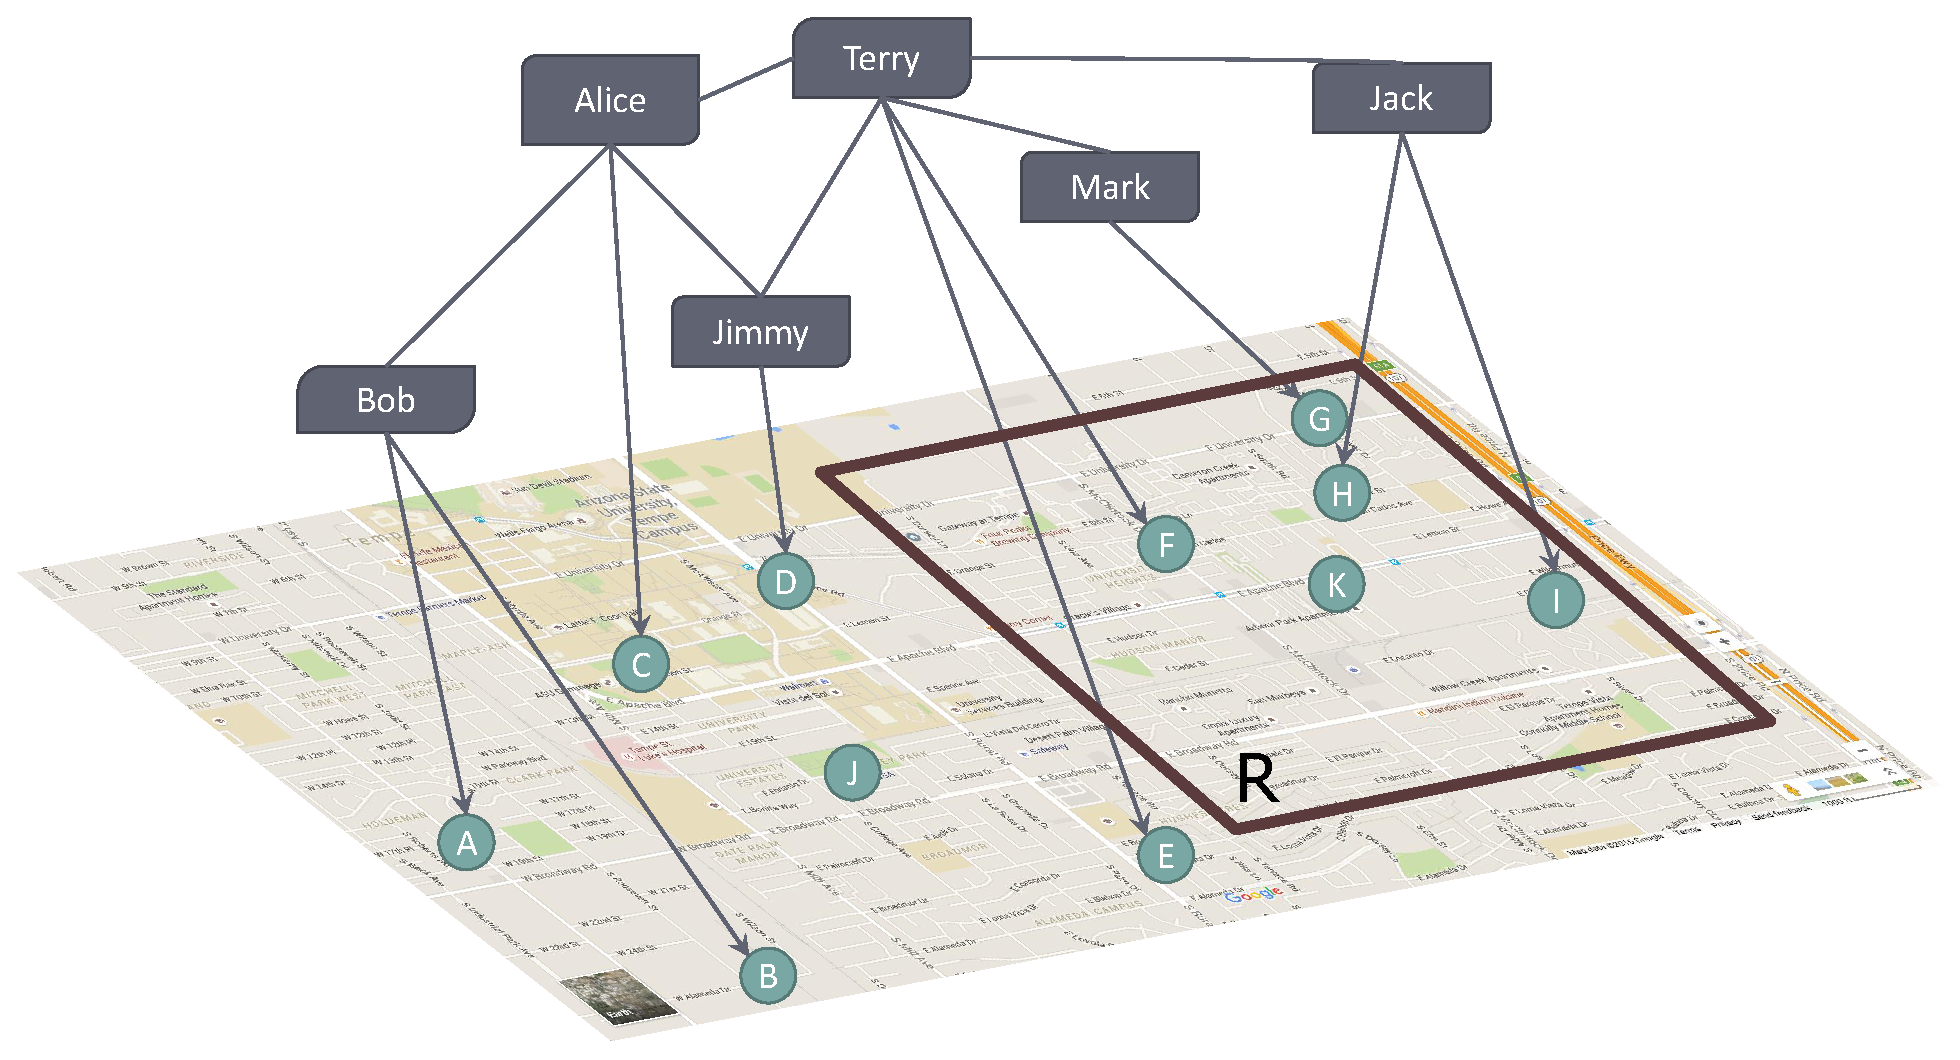
\includegraphics[width=0.88\linewidth]{images/a_motivation_example.eps}
	\caption{A motivation example}
	\label{fig:begin-example}
\end{figure}

And this paper is all about bringing these two even closer. We can predict what your best friend would have suggested to you if you wanted to go to an authentic Sushi place in SFO. Imagine restaurant recommendations from Google, are more personalized for a location instead of listing them by average user rating. To answer such queries it is required to traverse a social network and filter recommendations which fall in a given region. However minimum latency is rather imperative for such queries for the best user experience using huge social networks like Facebook, Twitter and Yelp. These graphs can be really dense, as much as, each person in the world is connected to every other person by only an average of three and a half other people!~\cite{Taa}. So the way to answer shortest path reachability queries with a spatial predicate quickly is needed even in such dense graphs (that is conditioned on a region).

Consider a restaurant recommendation system like Yelp. Every registered user can have multiple friends and also check-ins at multiple venues using this service. A small example from such a service would look like the one shown in Figure \ref{fig:begin-example} where Alice, Bob, Terry, Mark, Jack, Jimmy are people and letters from A to I are venues. Venues are also marked at the respective locations on a map. Edges between people indicate they are friends like in any social network and edges from a person to a restaurant means he/she checked-in at that location. Assume the system wants to recommend a restaurant to Bob in the marked region R and that all venues have the same average customer rating as 4.0. Any existing system would naturally return venues that fall in R in some random order as all of them are equally good. However, Bob is socially close to Terry than to Mark or Jack. Recommending restaurant F before G, H and I would make Bob happier as Terry and Bob are more similar in their tastes. Therefore, in order to provide good recommendations, we should consider both the spatial and social proximities in the search.

An easy way to solve the problem would be to find shortest distances to each venue falling in R, sorting them based on distance from the user of interest and picking the top K (whatever number is required). This disjoint approach can solve the problem but has a huge time latency especially while finding the closest vertices. Also we will be traversing huge graph aimlessly until we hit the required number of venues in R. Such a system would never be used in production. The paper~\cite{NSD2013} solves the problem in the disjoint manner using a distributed approach by implementing complex algorithms in a bottom up manner using simple distributed functions. This is a good start but we end up with other problems which distributed systems face today like network latency, consistency etc. The paper~\cite{KJY+2015} takes a new approach by combining the social and spatial constraints of the problem during the search routine but is more suited for queries like finding nodes close to a given node. However the aim is to find K closest vertices in a region from a (person) vertex in a social graph. So the big challenges ahead are to perform geosocial searches on huge graphs with (i) minimum latency, (ii) traverse the graph in a goal oriented manner towards the region unlike Dijkstra's, (iii) traverse the graph to the minimum as only the K closest vertices to a given vertex are required.

In this paper, we propose a new approach {\rrp} in order to solve {\query} query which finds top-k closest vertices to a given (person) vertex in a social graph considering both the social and spatial components. Our key contributions are as follows:
\begin{itemize}
	\item The paper studies the geosocial graph problem describing the challenge more formally and understand the need to solve this more efficiently.
	\item The paper proposes indices on social and spatial domains of the graph which form the pre-processing stage of the solution. Here graph data is stored in an organized manner to filter it based on spatial (region of interest) and social constraints (top-k closest vertices) at query time. This helps in solving the challenge of traversing to the minimum, as only best K are needed.
	\item The paper proposes a robust algorithm which uses above indices to answer top-k socio-spatial query using a modified landmark based A* algorithm by combining it with a spatial search. This solves the challenge of goal oriented search to reduce the latency even further.
	\item The paper experimentally evaluates the proposed approach with different parameter combinations on Yelp dataset. The experiments shows that our approach can achieve at least 3 times faster than existing approaches.
\end{itemize}

The rest of the paper is organized as follows: Section \ref{sec:relwork} demonstrates existing work related to {\rrp} and more insights on how our problem is different and why a better solution is required. In Section \ref{sec:preliminary} we formally define our problem in a more generic setting. Details of the proposed solution, including index structure, construction and cost analysis are given in Section \ref{sec:solution}. In Section \ref{sec:experiment} we evaluate our approach on a real dataset by comparing it with the baseline approach. Finally we conclude the paper and provide some future work in Section \ref{sec:conclusion}.


\section{Related Work to RRP(G, v, R)}
A naive solution to RRP can be to first find all vertices that fallinside R and then find shortest path to each. To filter vertices that fall inside R we can use a spatial index like a Quad tree or a R-tree. Then to find the shortest paths to each we can use an algorithm like Dijkstra's ~\cite{S1990} or Bellman Ford~\cite{R1956}. The paper~\cite{NSD2013} provides a distributed framework for this decoupled approach. They reduce a socio-spatial problem into smaller sub-problems and implement them as distributed functions.

Another idea is to combine the socio-spatial predicates for better pruning and paper~\cite{KJY+2015} proposes an idea where they prune the graph in a round robin manner by social and spatial distance functions. Using this algorithm we can answer queries like my friends who are socially and spatially closer to me.

{A lot of research has happened to answer reachability queries ranging from O($n^3$}{) memory intensive transitive closure algorithms to O($m \times n$) time intensive DFS and BFS algorithms. Approaches like GRAIL~\cite{YCZ+2010}, 2HOP~\cite{CHK+2003}, GRIPP~\cite{SU2007}, Dual Labeling~\cite{HHJ+2006} find a sweet spot between the two extremes to answer reachability and path queries. Here we are trying to find a pattern between a vertex and a spatial predicate region simultaneously and not between two vertices nor a path queries. }

There are several spatial indices~\cite{PMA2001,H2006,SS2003} that quickly filter a graph based on our spatial region. Some of them divide the space equally and some based on data. They recursively do this approach to construct a tree. This heavily improves the search speed as we prune a significant portion at every level as we traverse the tree. However, we can either create a tree for spatial vertices or for social vertices but not for both using ideas from these papers.

{The paper GeoReach~\cite{YM2016} gives an idea how to answer reachability queries with spatial predicate. They create an index with three types of vertices - B vertex, G vertex, R vertex with increasing degree of information about reachability to a region. The query returns true if a vertex can reach a region, else false. However, we need the entire path to a region and not just true or false.}


\section{Preliminary}
\label{sec:preliminary}

\begin{figure}[h]
	\centering
	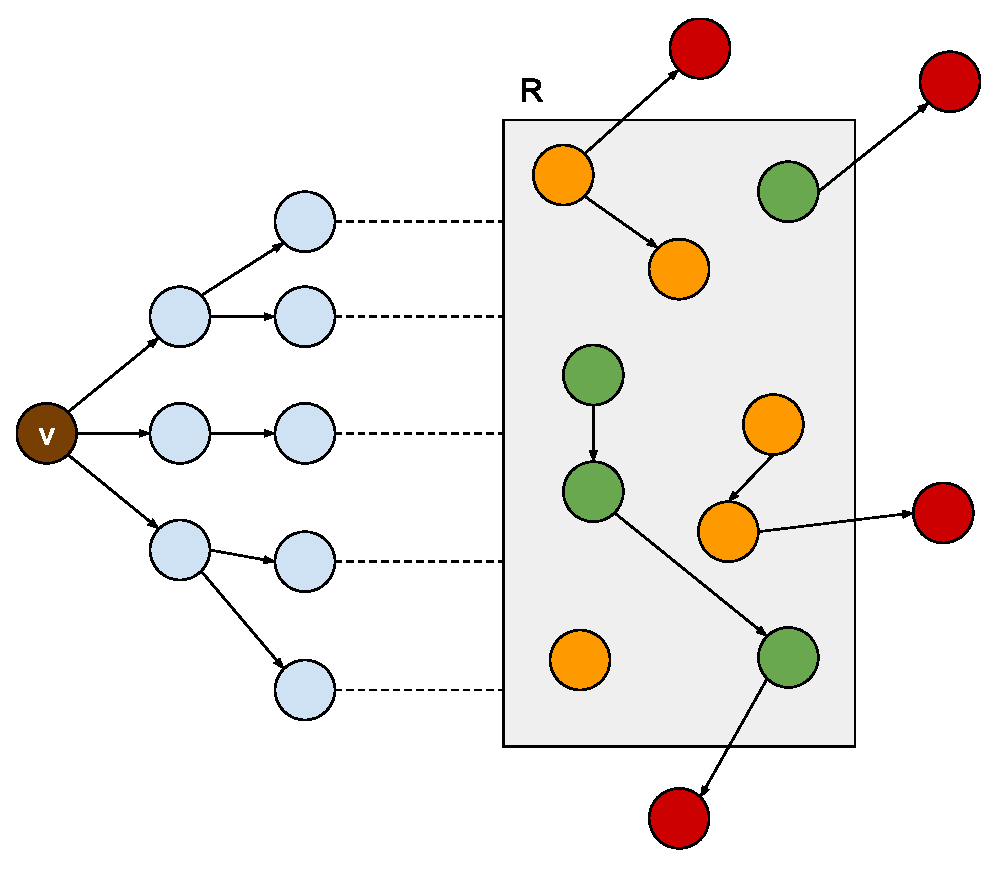
\includegraphics[width=0.88\linewidth]{images/a_social_graph.eps}
	\caption{A social graph showing friend-friend connections and also the region of interest}
	\label{fig:socio-spatial-graph}
\end{figure}

{\bf Graph Data.} A weighted directed graph $G=(V,E,S)$ consists of (1) a set of vertices $V$; (2) a set of directed edges $E\subset V\times V$ with weights. If $(u,v)\in E$, there exists one edge from vertex $u$ to $v$; (3) a function $S$ defined on $V$ that decides spatial attribute of a given vertex. $S(v)$ returns spatial property of $v$ (denoted as $v.spatial$) and the value will be null when $v$ brings no spatial attribute. $S(v)$ can be a geometrical a point, line, or polygon. For ease of presentation, we assume that a spatial attribute of spatial vertex is represented by a point.
%${\GeoReach} deals with a directed property graph $G=(V,E)$ where (1)~$V$ is a set of vertices such that each vertex has a set of properties (attributes) and (2)~$E$ is a set of edges in which every edge can be represented as a tuple of two vertices $v_1$ and $v_2$ ($v_1,v_2\in V$). The set of spatial vertices $V_S \subseteq V$ such that each $v \in V_{S}$ has a spatial attribute (property) $v.spatial$. The spatial attribute $v.spatial$ may be a geometrical point, rectangle, or a polygon. For ease of presentation, we assume that a spatial attribute of spatial vertex is represented by a point. Figure~\ref{fig:graph_example} depicts an example of a directed property graph. Spatial Vertices $V_S$ are represented by black colored circles and are located in a two-dimensional planer space while white colored circles represent regular vertices that do not possess a spatial attribute. Arrows indicate directions of edges in the graph.

\textbf{Path and Shortest Path.} A path is a sequence of vertices and edges that are distinct from one another. A path is denoted as $p =$ ($v_1$, $e_1$,..., $v_{n-1}$, $e_{n-1}$, $v_n$) where $v_i\neq v_j~and~e_i\neq e_j (i\neq j)$. Length of $p$ is denoted as $L(p) = \sum\limits_{i = 1}^{n-1}w(e_i)$. This path starts from vertex $v_1$ to $v_n$. In a weighted directed graph $G$, there possibly exists multiple paths between two vertices $u$ and $v$. $Paths(u,v) = \{p|p = (u,e_1,..., v)\}$ is to represent the set of all paths that start from $u$ and end at $v$. Shortest path between $u$ and $v$ is a path that has the shortest $L(p)$ where $p\in Paths(u,v)$, denoted as $ShortestPath(u,v)$.

\textbf{Shortest path between vertex and spatial region.} Given a vertex $v$ and a spatial region $R$, there exists many shortest paths between $v$ and each spatial vertex $u$ inside $R$, depending on how many spatial vertices are located in $R$. RangeReachShortestPath($v$, $R$, $k$) returns the $k$ shortest paths among all shortest paths between $v$ and $u$.

\iffalse
Given a graph $G(V, E)$ where,

\quad$V \rightarrow set\ of\ vertices$

\quad$E \rightarrow set\ of\ edges$

$Vs \subset V$ have spatial attributes; i.e. $\forall v \in Vs \Leftrightarrow v.spatial$ attribute exists\\


\textbf{RangeReachPaths S(G, v, R):} a set of shortest paths starting from v that reach a region R in graph G, where R is a spatial range predicate. Let's abbreviate this as RRP(v, R).

\textbf{Path, P(u, w):} A set of vertices along the way from u to w \(\Rightarrow w\ is\ reachable\ from\ u\)

\quad${P(u, w) \in S(v, R) \Leftrightarrow}$

\quad\quad{u = v and}

\quad\quad${w \in Vs}$ and

\quad\quad{w.spatial lies in region R}\\

\fi

Figure \ref{fig:socio-spatial-graph} pictorially represents the entire problem. v is the source vertex and R is the region of interest. Red, green and yellow vertices have spatial attributes like latitude and longitude information. Red vertices fall outside the region and so are not returned by RRP. Yellow vertices fall inside R but cannot be reached from v, so are not returned by RRP. Green vertices satisfy both these conditions as they fall inside the region and are also reachable from v. ~Therefore, RRP returns the paths to all green vertices. These paths with rich social information about the relationship with v, can be fed into a recommendation system which can rank them.

\iffalse
\begin{figure}[h]
    \centering
    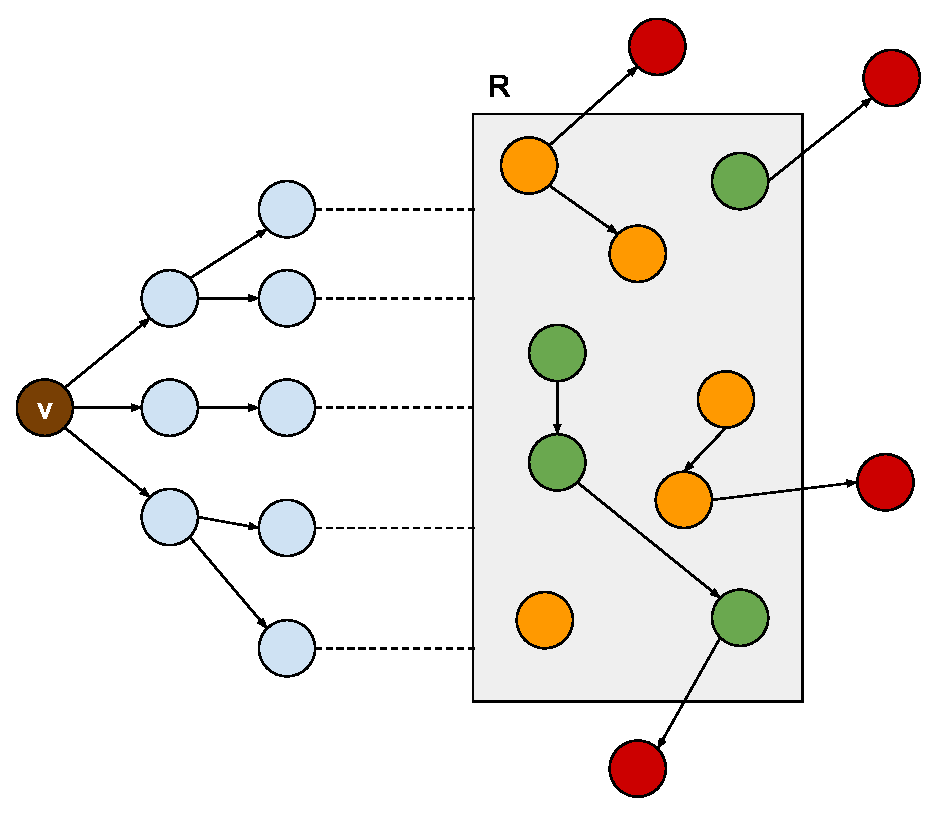
\includegraphics[width=0.5\linewidth]{images/image10.eps}
    \caption{A social graph showing friend-friend connections and also
the region of interest}
    \label{fig:socio-spatial-graph}
\end{figure}

Figure \ref{fig:socio-spatial-graph} pictorially represents the entire problem. v is the source vertex and R is the region of interest. Red, green and yellow vertices have spatial attributes like latitude and longitude information. Red vertices fall outside the region and so are not returned by RRP. Yellow vertices fall inside R but cannot be reached from v, so are not returned by RRP. Green vertices satisfy both these conditions as they fall inside the region and are also reachable from v. ~Therefore, RRP returns the paths to all green vertices. These paths with rich social information about the relationship with v, can be fed into a recommendation system which can rank them.
\fi

\section{Our approach: {\orirrp}} \label{sec:solution}
{\rrp} is a modified A* algorithm with better pruning power. {\rrp} consists of two main components - spatial and social. Spatial component is a grid-based index for pruning graph branches while the social component uses landmark technique to generate distance heuristic for guiding graph traversal. The following sections talk about them in more detail.
%The solution is two fold, first data is preprocessed to create an index. Then a modified A* algorithm traverses the graph using the index to answer query of type mentioned in Section \ref{sec:preliminary}.

% Throughout the section, a running example is used to explain the main idea followed by a formal algorithm. Consider Figure \ref{fig:running-example-solution} which has a social graph of friends and their check-ins at various venues. In Figure \ref{fig:running-example-solution}, each vertex symbolizes a person and two nodes are connected if there is a social relationship between them. The number on the edge indicates their social distance, lesser implies stronger bond. Forest green edges from the nodes to the map are all check-ins made by people at various venues (nodes not shown), which are our spatial vertices. Forest green edges are also weighted but are not shown as they are not important for explanation purposes.

\begin{figure}[t]
	\centering 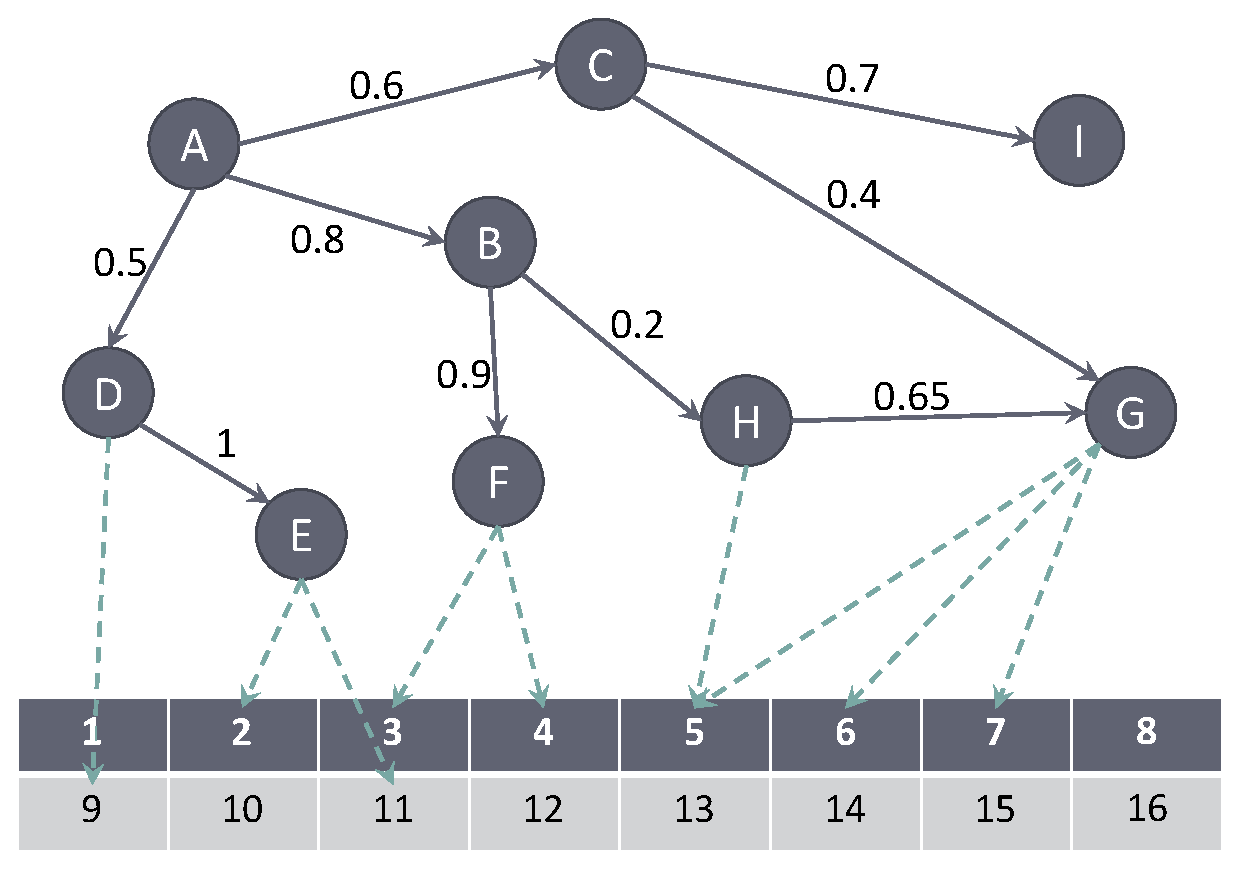
\includegraphics[width=0.40\textwidth]{images/space_partitioned_world.eps}
    \caption{Running Example}
    \label{fig:running-example-solution}
\end{figure}

%\subsection{Index Structure}
%Goal of the index is to quickly prune the graph for any range predicate, starting at any source vertex. Therefore for every vertex, spatial and social meta information is added. Using this meta information, the traversal algorithm at query time can decide whether to visit a sub-graph starting at that node or not or more generally, this guides the traversal algorithm at query time.

%Spatial meta information is created using the spatial attributes of the vertices. The world is divided into a fixed number of blocks in space and are numbered in increasing order. Then for each venue (i.e. spatial node) the meta information for all the people nodes (other vertices) who have directly and indirectly checked-in there is updated with the block number where the venue belongs. 

% If the world is divided into very fine blocks, each meta entry can be really huge. To compress the index entry, the world is divided again but this time into more coarser blocks and are also numbered like before. For all the index entries which cross a threshold, block numbers from the coarser division are used. This is done recursively until the threshold is satisfied for that index entry. Once this is in place, at query time, while traversing the graph for finding a closest vertex, sub-graphs starting at a vertex which does not reach the region of interest are straight away pruned.

%Social meta information/index is created using the social distances (edge weights). A few vertices are picked from the graph and the shortest distances from each to all vertices it can reach are stored. Using these vertices and triangle inequality an estimate of the shortest distance from any vertex to any other vertex in the graph is obtained.

\subsection{Spatial Component}

\begin{figure}[t]
	\centering \includegraphics[width=0.40\textwidth]{images/entire_world_grid.eps}
    \caption{Space partitioned world}
    \label{fig:space-partitioned}
\end{figure}

A complete picture of equally space partitioned world would be as shown in the Figure~\ref{fig:space-partitioned}. Here the resolution of the division is 10 by 10. In the running example, the entire region is divided into equal sized blocks from 1 to 16 as shown in Figure \ref{fig:running-example-solution}. Then for vertex D, meta information would be [8] as the user checked-in at a venue which falls in block number 8. Similarly for vertex G, the meta information would be [5, 6, 7]. Continuing like this, a meta information table for each vertex which are directly connected to a spatial node is populated.
%A complete picture of equally space partitioned world would be as shown in the Figure~\ref{fig:space-partitioned}. Here the resolution of the division is 10 by 10. That means the entire world is divided into 10 equal sized blocks horizontally and 10 equal sized blocks vertically. In the running example, the entire region is divided into equal sized blocks from 1 to 16 as shown in Figure \ref{fig:running-example-solution}. Then for vertex D, meta information would be [8] as the user checked-in at a venue which falls in block number 8. Similarly for vertex G, the meta information would be [5, 6, 7]. Continuing like this, a meta information table for each vertex which are directly connected to a spatial node is populated.

% \begin{table}[h]
% 	\caption{1-hop reachability meta table}
% 	\label{tab:1-hop-meta}
% 	\begin{center}
% 		\renewcommand{\arraystretch}{1.25}
% 		\begin{tabular}{ c | c }
% 			\hline
% 			Vertex & Reachable Block Numbers \\ \hline
% 			\hline
% 			D & [8] \\
% 			E & [2, 10] \\
% 			F & [3, 4] \\
% 			H & [5] \\
% 			G & [5, 6, 7] \\
% 			\hline
% 		\end{tabular}
% 	\end{center}
% \end{table}

% This is the reachability to venues by 1-hop which can answer 1-hop queries. For example, did vertex G check-in at venue L1 or did vertex E visit any venue in a region L2. The first can be answered by finding its block number using its location and cross-reference it with the list of blocks G can reach from the meta table. More details on answering queries are in Section \ref{querying}.

% If idea of 1-hop reachability is extended to any number of hops, it is multi-hop reachability or simply reachability. These values denote all blocks that are reachable from a vertex in any number of hops/steps. 

Now to complete building the reachable block table, direction of all the edges are reversed or the transpose of a graph is created. Then, for every vertex, its reachability information is appended with meta information of all the vertices it is directly connected to bottom up. In the example after reversing the edges, to compute multi-hop meta information for H, append G's meta information to it. Similarly for B's meta information is appended from H and F. As this is a DAG, this is the complete reachability information of every node after completing the exercise for entire graph. If the original graph is not a DAG, it is condensed by contracting all strongly connected components into a single node to make it a DAG. The final meta table for every node looks like the one shown in the column 2 of Table \ref{tab:multi-hop-meta}.

\begin{table}[h]
	\caption{Meta table for multi-hop reachability}
	\label{tab:multi-hop-meta}
	\begin{center}
		\renewcommand{\arraystretch}{1.25}
		\begin{tabular}{ c | c | c }
			\hline
			Vertex & Reachable Block Numbers & Compressed\\ \hline
			\hline
			D & [9, 2, 11] & [17, 18] \\
			E & [2, 11] & [2, 11] \\
			F & [3, 4] & [3, 4] \\
			H & [5, 6, 7] & [19, 20] \\
			G & [5, 6, 7] & [19, 20] \\
			C & [5, 6, 7] & [19, 20] \\
			B & [3, 4, 5, 6, 7] & [21] \\
			A & [3, 4, 5, 6, 7] & [21] \\
			\hline
		\end{tabular}
	\end{center}
\end{table}

Using this table any region reachability query can be answered and will be described in Section \ref{querying}. Now it can seen that vertex A can reach whatever B, C and D can reach. Similarly B can reach whatever H and F can reach and so on. However, as you can see the size of the meta table (a.k.a index table) can grow really large as vertices like B and A which are highly connected can reach many blocks.

In order to compress the entries in the meta table for highly reachable nodes, a new layer of blocks with higher resolution is added.

% \begin{figure}[h]
%     \centering
%     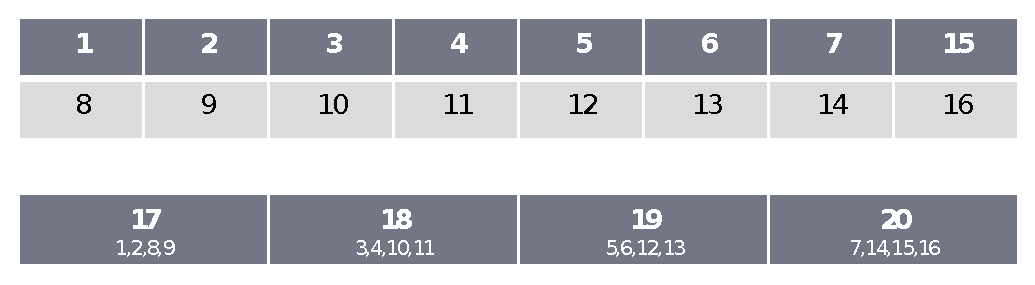
\includegraphics[width=0.8\linewidth]{images/image07.eps}
%     \caption{Multi layer grid index}
%     \label{fig:multi-grid}
% \end{figure}

As shown in Figure \ref{fig:multi-grid2} (assume the 3rd layer does not exist for now), blocks 17 to 20 are added on top of blocks 1 to 16. This can be visualized like a stack where the old layer sits exactly on top of the new layer. That is block 17 covers exactly the same area as area covered by blocks 1, 2, 8 and 9. Similarly block 18 in layer 1 represents blocks 3, 4, 10 and 11 of layer 0. Due to this change, the meta table becomes like the one shown in the 3rd column of the Table \ref{tab:multi-hop-meta}. The reduction factor, which is rate at which the resolution changes between adjacent layers, is set to 1/4 and is a tunable parameter of the system called RF. The number of layers in the multi layer grid index is guided by another system level tunable parameter M. M is the maximum size, in terms of number of block ids, of meta information for a vertex. For example, if M = 2 as used in the running example, then each vertex can only have two entries in its meta information and until this limit is satisfied, new layers are created. In the example, for all vertices which have more than 2 entries, are compressed using layer 1. However some of them still have more than 2 entries. 

% \begin{table}[h]
% 	\caption{Compressed Meta table for multi-hop reachability}
% 	\label{tab:multi-hop-meta-compressed}
% 	\begin{center}
% 		\renewcommand{\arraystretch}{1.25}
% 		\begin{tabular}{ c | c }
% 			\hline
% 			Vertex & Reachable Block Numbers \\ \hline
% 			\hline
% 			D & [8] \\
% 			E & [2, 10] \\
% 			F & [3, 4] \\
% 			H & [\textbf{19, 20}] \\
% 			G & [\textbf{19, 20}] \\
% 			\textbf{C} & [\textbf{19, 20}] \\
% 			\textbf{B} & [\textbf{18, 19, 20}] \\
% 			\textbf{A} & [\textbf{18, 19, 20}] \\
% 			\hline
% 		\end{tabular}
% 	\end{center}
% \end{table}

To compress further one more layer below layer 1 is added as show in Figure \ref{fig:multi-grid2}. There block 21 represents blocks 17, 18, 19 and 20 in the layer above it. 

\begin{figure}[t]
    \centering
    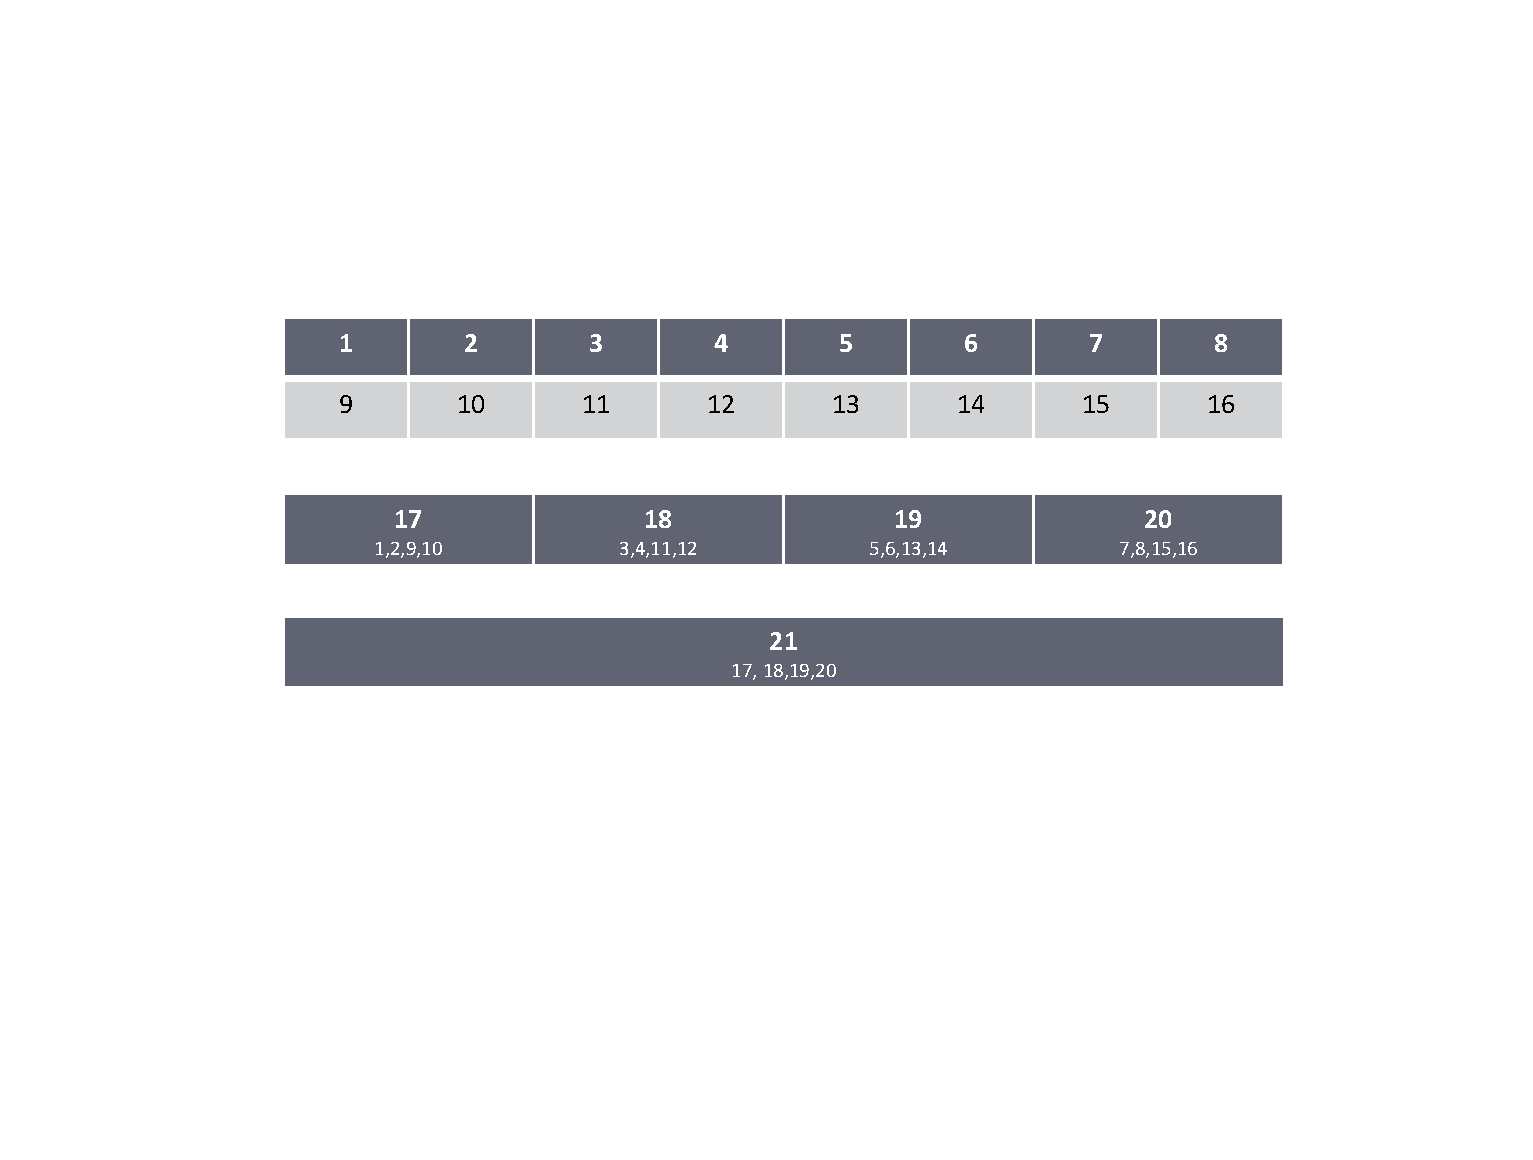
\includegraphics[width=0.88\linewidth]{images/multi_layer_grid_index.eps}
    \caption{Multi layer grid index}
    \label{fig:multi-grid2}
\end{figure}

The discussion began by condensing G to a DAG (G'). Now each node in a strongly connected component gets the meta information of the component as proved Lemma \ref{vertex-component-meta}.

\begin{lemma}
\label{vertex-component-meta}
Let v be a vertex in a strongly connected component C of a directed graph G(V, E). Then,

{\{$\forall v \in C$: Meta information of v = Meta information of C\}}\\
\end{lemma}

\begin{proof}
In a strongly connected component $C$, any vertex can be reached from any vertex by definition, i.e. $u \leadsto v, \forall (u, v) \in C$. 

If $C$ in condensed graph $G'$ can reach a set of regions $R$, then any vertex of $C$ can reach $R$ by definition of connected component.

Therefore, meta information of $C =$ meta information of $\forall v \in C$
\end{proof}

Then a R-Tree is also constructed using the spatial nodes in the graph. This will later be used at query time to filter the exact nodes in a region and will be discussed in more details in Section \ref{querying}. R-Tree index and reachable blocks table are the two indices created on the spatial component of the graph.

Algorithm \ref{alg1} shows how the index, {\rrpspatial} is created. In the first phase block numbers of all spatial vertices are added as the meta information of the vertices they are connected from. Then a modified DFS is used to construct multi hop reachability. The REGION() method returns the block number for any spatial vertex. The REPARTITION() method ensures the M constraint by recursively increasing the resolution by a factor of RF. In the DFS() method meta information is recursively appended to the head vertex from the tail vertex.

% \begin{algorithm*}[h]
% \caption{{\grpspatial}}
% \label{alg1}
% \begin{multicols}{2}
% \begin{algorithmic}[1]
% \State $MIN\_LAT \gets -90$
% \State $MAX\_LAT \gets 90$
% \State $MIN\_LNG \gets -180$
% \State $MAX\_LNG \gets 180$
% \State $DEFAULT\_RES \gets 10$ \Comment{Can be any positive integer}
% \State $AVAILABLE\_RES \gets [DEFAULT\_RES]$
% \State
% \Function{{\grpspatial}}{$G, RF, M$}
%   \State $G' \gets DAG(G)$
%   \For{$v \gets G'.v:$}
%   	\State $v.meta \gets Set([])$   	\Comment{Initialize an empty set}
%   \EndFor
%   \State
%   \For{$u \gets spatial(G'.Adj(v))$}	 \Comment{1\-hop spatial reachability}
%   	\State v.meta.add(\Call{REGION}{u})
% 	\State \Call{REPARTITION}{v, RF, M}
%   \EndFor
%   \State
%   \State DO\_DFS(G', RF, M)  \Comment{multi\-hop region reachability}
% \EndFunction
% \State
% \Function{REGION}{$u$}
% 	\State $r \gets GET\_RES(u)$
% 	\State $cols \gets (MAX\_LAT - MIN\_LAT) \div r$
% 	\State \Return $floor(u.x \div r) + floor(u.y \div r)$
% \EndFunction
% \State
% \Function{REPARTITION}{$v, RF, M$}
% 	\If{$v.meta.size() \leq M$}
% 		\State \Return
% 	\EndIf
% 	\State $res \gets GET\_RES(v.meta[0])$
% 	\For{$r \gets v.meta$}
% 		\State \Call{TRANSLATE\_TO\_RES}{v.meta, $res \div MF$}
% 		\State \Call{REPARTITION}{v, RF, M}
% 	\EndFor
% \EndFunction
% \State
% \Function{DO\_DFS}{G, RF, M}
% 	\For{$v \gets G,V$}
% 		\State $v.visited \gets false$
% 	\EndFor
% 	\State
% 	\For{$v \gets G.V$}
% 		\State v.meta.add(\Call{DFS\_VISIT}{G, v})
% 		\State \Call{REPARTITION}{v, RF, M}
% 	\EndFor
% \EndFunction
% \State
% \Function{DFS\_VISIT}{G, v}
% 	\For{$u \gets G.Adj(v)$}
% 		\If{$v.visited = false$}
% 			\State v.meta.add(\Call{DFS\_VISIT}{G, u})
% 		\Else
% 			\State v.meta.add(u.meta)
% 		\EndIf
% 		\State \Call{REPARTITION}{v, RF, M}
% 		\State $v.visited \gets true$
% 		\State \Return v.meta
% 	\EndFor
% \EndFunction
% \end{algorithmic}
% \end{multicols}
% \end{algorithm*}

\begin{algorithm}[t]
\caption{{\rrpspatial} Initialization}
\begin{scriptsize}
\label{alg1}
\begin{algorithmic}[1]
\Function{{\inirrpspatial}}{$G, RF, M$}
  \State G' $\gets$ G.condense() \label{alg:condense}
  \For{v $\gets$ G.V} \Comment{1\-hop spatial reachability} \label{alg:onehopstart}
	  \For{u $\gets$ spatial(G'.Adj(v))}	 
	  	\State v.meta.add(\Call{REGION}{u})
	  \EndFor
	  \State \Call{REPARTITION}{v, RF, M}
  \EndFor \label{alg:onehopend}
  \State DO\_DFS(G', RF, M)  \Comment{multi\-hop region reachability} \label{alg:dfs}
\EndFunction
\Function{REGION}{$u$}
	\State \Return block \# for CURRENT\_RES(u)
\EndFunction
\Function{REPARTITION}{$v, RF, M$}
	\While{$v.meta.size() \leq M$}
		\State \Call{TRANSLATE\_TO\_RES}{v.meta, CURRENT\_RES(v) $\div$ RF}
	\EndWhile
\EndFunction
\Function{DO\_DFS}{G, RF, M}
	\For{$v \gets G.V$}
		\State v.meta.add(\Call{DFS\_VISIT}{G, v})
		\State \Call{REPARTITION}{v, RF, M}
	\EndFor
\EndFunction
\Function{DFS\_VISIT}{G, v}
	\For{$u \gets G.Adj($v) not $visited$}
		\State v.meta.add(\Call{DFS\_VISIT}{G, u})
	\EndFor
	\State \Return v.meta
\EndFunction
\end{algorithmic}
\end{scriptsize}
\end{algorithm}

To compute the asymptotic run time and space complexities for Algorithm \ref{alg1}, it is divided into four pieces - graph condensation, reachability and repartition function. The runtime for each would be as follows,
\begin{itemize}

  \item \textbf{Graph Condensation}: On Line~\ref{alg:condense}, the input graph is condensed into its strongly connected components. Using a popular algorithm like Targan's Algorithm, the runtime would be $O(V + E)$~\cite{R1972}.

  \item \textbf{Reachability calculation}: From lines~\ref{alg:onehopstart} to~\ref{alg:dfs}, reachability on the condensed graph is computed. In the worst case, every vertex will be a strongly connected component and so the size of the graph remains the same after graph condensation. As the entire graph is traversed once to populate meta data for each vertex, the complexity for this piece also would be $O(V + E)$. Calls to repartition() function are handled separately.

  % \item \textbf{DFS}: For multi-hop reachability, a DFS traversal is performed on the graph on Line~\ref{alg:dfs}. As adjacency list is used for managing the graph's edges, the complexity for DFS would be $O(V + E)$ again. Calls to repartition() function are handled separately.

  \item \textbf{Repartition}: This function is called multiple times to make sure the M constraint is satisfied. The runtime of the function depends on the size of the meta entry for the vertex. For every vertex's index entry, the world is divided with a constant resolution to start with, like 10. The total number of blocks at that default resolution would always be square of it, like 100. Let the total number of blocks in the default resolution be $c$, which would be the worst case size of any vertex's meta information. This happens when a vertex can reach all blocks in the world. And until the size of meta information for that vertex falls below M, the resolution of the division is reduced by $RF$. Therefore the number of times the loop in REPARTITION() function of the algorithm, say $n$ would be,

  \begin{eqnarray*}
  	\dfrac{c}{RF^n} \leq M\\
  	n \leq {\log_{\dfrac{1}{RF}} (\dfrac{M}{c})}
  \end{eqnarray*}
  And repartition function is called exactly twice for each vertex, once during 1-hop reachability and once during DFS. Therefore, the time complexity due to this function would be $O(V \times {\log_{\dfrac{1}{RF}} (\dfrac{M}{c})})$. This fraction is very small compared to sum of vertices and edges in the graph.
\end{itemize}

All the other lines in the algorithm can be computed in constant time. The runtime of {\rrpspatial} would hence be $O(V + E)$.

Space complexity would be amount of memory required to store the multi-hop reachability table. Each index entry has an upper bound of $M$. Hence memory consumption in the worst case would be, $O(V \times M)$.

\subsection{Social component}
Social distances between nodes are used to create an additional index to prune the graph even better. This will take care of the cases when the graph is very dense and the spatial reachable blocks table created before may not be of much use for pruning at query time. More details on querying the graph are described in the next section.

The main idea is to select a few nodes in the graph and call them landmarks. Then for each vertex shortest distances to each landmark is stored. Then at query time these precomputed distances and triangle inequality are used to guide as a heuristic in the A* search algorithm. The inspiration is from \cite{AC2005} which introduces a class of algorithms called ALT. The main challenge here however is to find top-k closest vertices to a given vertex in a region and not finding the shortest path from a given source to a given destination unlike in \cite{AC2005}.

The quality of the landmarks determine the pruning power of the index. Choosing the right landmarks requires some domain knowledge of the graph. Once that is picked the process remains the same no matter what the graph represents. \cite{AC2005} talks about multiple ideas on how to find high quality landmarks quickly. The ideal case would be to find as minimum number of landmarks as possible such that every vertex in the graph is connected to at least one of the landmarks.  However leaving out a few vertices that do not reach any landmarks will not hamper the correctness of the algorithm. Therefore finding a sweet spot of number of landmarks which gives the best query performance is crucial and is the main goal of \cite{AC2005}. The main contribution from our side is to use {\rrpsocial} and propose a new heuristic for A* algorithm that finds topK venues satisfying a spatial predicate.

Algorithm \ref{alg2}, {\rrpsocial}, describes how to create an index using landmarks. Landmark selection function on line 2 can be any of the functions described in \cite{AC2005}. Then for each landmark the shortest distances is computed using any well-known single source shortest path algorithms like Dijkstra's or Bellman Ford to every vertex reachable from that landmark. Please note that distances from the landmark to every vertex are saved and not the other way around. The direction is important as directed graphs are only dealt here.

\begin{algorithm}[t]
\caption{{\rrpsocial}  Initialization}
\begin{scriptsize}
\label{alg2}
\begin{algorithmic}[1]

\Function{{\inirrpsocial}}{$G$}
  \State L $\gets$ FIND\_LANDMARKS(G) \Comment{Domain based}
  \State social\_index $\gets$ []
  \For{l $\gets$ L}
    \For{v $\gets$ G.v}
	  	\State social\_index[l][v] $\gets $ shortest distance from l to v
	\EndFor
  \EndFor
\EndFunction
\end{algorithmic}

\end{scriptsize}
\end{algorithm}

To compute asymptotic run time and space complexities, Algorithm \ref{alg2} is divided into two pieces - finding the landmarks, finding shortest distances to each reachable vertex from each landmark. The runtime for each is as follows,
\begin{itemize}
	\item \textbf{Finding Landmarks}: There are various ways of picking the landmarks and is totally left to user. In our case we used an approach which finds landmarks in constant number of scans of the entire graph. Therefore, the complexity of this piece is $O(V + E)$.

	\item \textbf{Shortest distance to each landmark}: Here, the shortest distances from each landmark to all vertices it can reach are saved. Using adjacency list for storing the edges, Dijkstra's algorithm is used as edges have positive weights. With this setting, the complexity would be $O(landmarks \times E\log V)$. As the number of landmarks is usually very small compared to number of edges in the graph, it would be $O(E\log V)$ in asymptotic notation.
\end{itemize}

Therefore the runtime for this algorithm using a sensible landmark selection algorithm would be, $O(V + E) + O(E\log V)$.

Space complexity would be memory taken to store the shortest distances to each reachable vertex for all landmarks. As the number of landmarks is very small compared to the number of vertices in the graph, this would be $O(V)$.

\subsection{Query Processing} \label{querying}

A modified A* with landmark~\cite{AC2005} algorithm is proposed for answering {\query} queries using the {\grp} index ({\rrp}). The main goal is to prune as much graph as possible using the spatial reachable blocks table and move in a goal oriented manner towards the region during traversal. The algorithm takes a graph G, a starting vertex s and a query rectangle R as input and returns the top-K vertices by social distance in R in an iterative manner. Being iterative helps pipeline the {\rrp} with other database functions.

The crux of A* algorithm is the heuristic function. Our heuristic function takes a vertex and a region and returns the heuristic distance which will be used by A* to decide which path to traverse. In order to design such heuristic function {\rrpsocial} index is used explained in Algorithm \ref{alg3}. For this the triangle inequality property is used to get a lower bound on the distance between any two vertices.

In Figure \ref{fig:tri-ine}, say $H$ and $R$ vertices need a lower bound on the distance between them. For this, the distances saved w.r.t. each landmark, here $G$ as part of social {\rrp} index is used. So in the figure using the index the distances \textbf{u} and \textbf{v} are known. In order to find \textbf{x} which is the distance between $H$ and $X$ \textbf{u} is subtracted from \textbf{v}. Therefor the value of \textbf{x} shown in the figure would be $\textbf{v} - \textbf{u}$ which directly follows from vector addition. This is only a lower bound on the distance from $H$ to $X$ and is proved in \cite{AC2005}.

In our case a lower bound from a vertex to a region is needed. In order to understand how this is done, recap the problem definition - find top-k closest vertices (w.r.t social distances) in a region from a vertex in a graph. To understand better, set K = 1, i.e. say the nearest vertex in the R from a source vertex is needed and say only one landmark is present. Now, for A* to work efficiently, a lower bound as tight as possible is needed, else the traversal would touch as many vertices as Dijkstra's. Let the source vertex be $H$, landmark be $G$ and region exactly enclosing blocks 5 and 6 in the Figure \ref{fig:tri-ine}. The problem now becomes finding the closest vertex to $H$ in the region. To get a lower bound for $\textbf{x}$, the triangle inequality formula devised above, $\textbf{v} - \textbf{u}$ is used. In order to keep $\textbf{x}$ minimum, $\textbf{v}$ should be as small as possible. Therefore the closest vertex in R to $G$ is picked. Similarly for the second closest vertex the second nearest vertex to $G$ in R is chosen. The algorithm proceeds this way till the nearest K vertices in R are found. If multiple landmarks are present, a value of \textbf{x} for each landmark is produced. The maximum value of \textbf{x} is picked to get the tightest bound possible and this follows from efficiency of A* algorithm.

\begin{figure}[t]
    \centering
    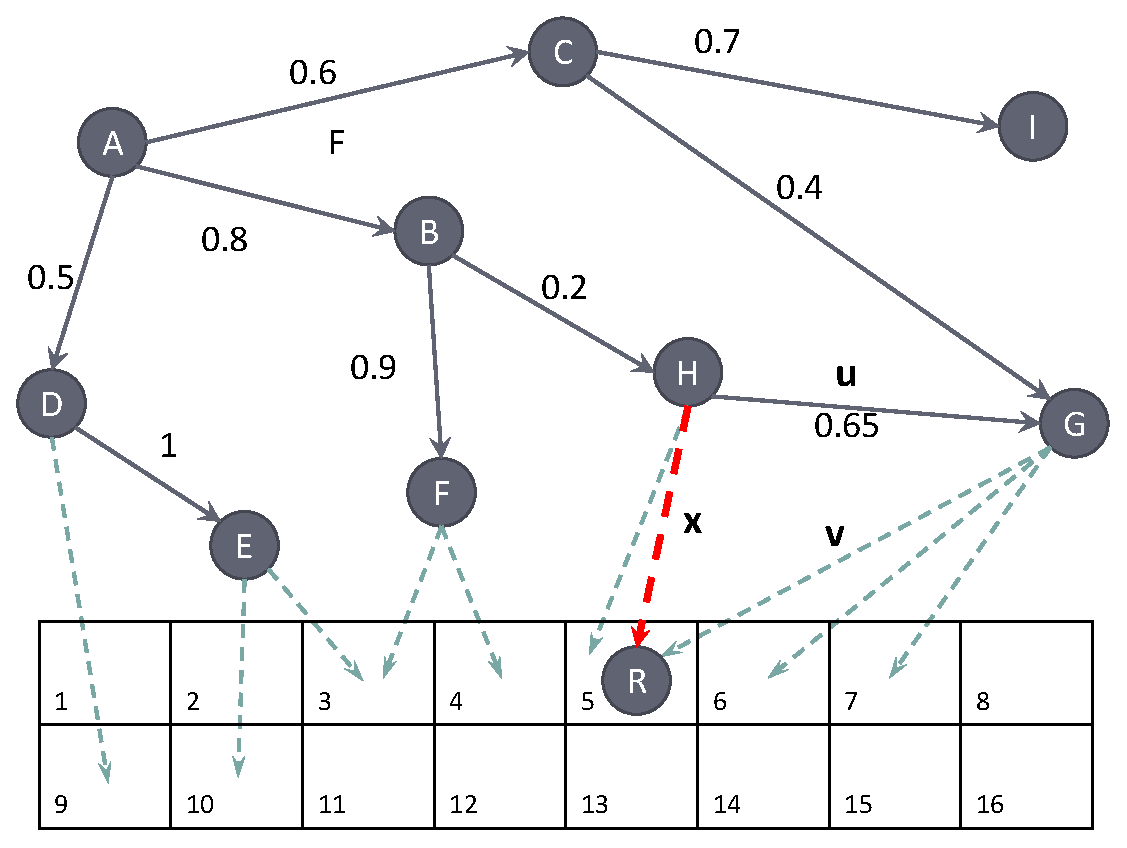
\includegraphics[width=0.88\linewidth]{images/triangle_inequality.eps}
    \caption{Triangle Inequality}
    \label{fig:tri-ine}
\end{figure}

Algorithm \ref{alg3} shows how to solve {\query} by using {\rrp} in detail. All vertices are labelled as unvisited initially. The visited flag is used to prevent traversing the same node multiple times. The priority queue $Q$ in keyed by sum of actual distance from source and a heuristic distance to current closest vertex to a landmark. For each vertex popped from the queue, it is tested if it lies in R and returned if K vertices are found. If not, keys for all existing vertices in Q are updated with the new heuristic. All unvisited neighbors of the popped vertex are enqueued only if they can reach the region R as per {\rrpspatial} index. If a neighbor can reach R, and if it not already in $Q$, its heuristic distance is computed and summed with the distance from the source and inserted into the $Q$. If the vertex is already in the $Q$, its key is updated if the new distance is smaller. The algorithm proceeds this way till all vertices in the Q are exhausted or K closest vertices in R are found whichever is earlier. This way, it is an iterative algorithm which doesn't traverse the entire graph to return the top-K results.

% \begin{algorithm*}[h]
% \caption{RangeReachPaths}
% \label{alg2}
% \begin{multicols}{2}
% \begin{algorithmic}[1]
% \Function{{\rrp}}{G, s, R, K}
% 	\State $nearest\_vertices \gets []$
% 	\State \Call{INIT}{G, s}
% 	\State $Q \gets [s]$
% 	\State $best\_index \gets 0$
% 	\While{Q is not empty}
% 		\State $v \gets \Call{EXTRACT\_MIN}{Q}$
		
% 		\If{\Call{LIES\_IN}{v, R}}
% 			\State $nearest\_vertices << v$ \Comment{add v to set}
% 			\State $best\_index \gets best\_index + 1$
% 			\If{nearest\_vertices.length = K}
% 				\State \Return \Call{PATHS}{nearest\_vertices}
% 			\EndIf
% 			\For{$v \gets Q$} \Comment{Update heuristic for existing in Q}
% 				\State $v.key \gets v.d +$ HEURISTIC(u, R, best\_index)
% 			\EndFor
% 		\EndIf
		
% 		\If{v.color = WHITE}
% 			\State $v.color \gets$ BLACK
% 			\For{$u \gets G.Adj(v)$}
% 				\If{\textbf{not} \Call{LIES\_IN}{R, GRP-SPATIAL(u)}}
% 					\State \textbf{continue}
% 				\EndIf
% 				\If{u.color = WHITE}
% 					\If{u in Q}
% 						\If{u.d < v.d + WEIGHT(u, v)}
% 							\State \textbf{continue}
% 						\Else
% 							\State $u.key \gets v.d +$ WEIGHT(u, v)
% 						\EndIf
% 					\Else
% 						\State $u.parent \gets v$
% 						\State $u.d \gets v.d +$ WEIGHT(u, v)
% 						\State $u.key \gets HEURISTIC(u, R, best\_index)$
% 						\State Q.INSERT(u)
% 					\EndIf
% 				\EndIf
% 			\EndFor
% 		\EndIf
% 	\EndWhile
% \EndFunction
% \State

% \Function{HEURISTIC}{u, R, i}
% 	\State $v \gets RTREE.filter(R)$   	\Comment{vertices in R}
% 	\State \Return MAX( MIN$_i$(GRP-SOCIAL(l, u) $\forall u \in v) \forall l \in$ L)
% 	\State \Comment{$i^{th}$ minimum $u$ in $v$}
% \EndFunction
% \State

% \Function{INIT}{G, s}
% 	\State $s.key \gets 0$   	\Comment{key for priority queue}
% 	\State $s.d \gets 0$	\Comment{actual distance from source}
% 	\For{$v \gets G.V$}
% 		\State $v.color \gets$ WHITE 
% 		\State $v.parent \gets NULL$
% 	\EndFor
% \EndFunction
% \State

% \Function{LIES\_IN}{x, y}
% 	\If{x is a region}
% 		\If{x overlaps or completely falls in y}
% 			\State \Return true
% 		\EndIf
% 	\EndIf
% 	\If{x is a point \textbf{and} x falls in y}
% 		\State \Return true
% 	\EndIf
% 	\State \Return false
% \EndFunction
% \State

% \Function{PATHS}{vertices}
% 	\State $ps \gets []$ \Comment{list of paths for all vertices}
% 	\For{$u \gets vertices$}
% 		\State $p \gets []$
% 		\While{u.parent <> NULL}
% 			\State $p.prepend(u)$
% 			\State $u \gets u.parent$
% 		\EndWhile
% 		\State $p.prepend(u)$
% 		\State $ps << p$
% 	\EndFor
% \EndFunction
% \end{algorithmic}
% \end{multicols}
% \end{algorithm*}

\begin{algorithm}[t]
\caption{{\query} Query}
\begin{scriptsize}
\label{alg3}
\begin{algorithmic}[1]
\Function{{\query}}{G, s, R, K}
	\State $nearest\_vertices \gets []$
	\State $Q \gets [s]$
	\State $best\_index \gets 0$
	\While{$Q$ is not empty}  \label{alg:theqstart}
		\State $v \gets \Call{EXTRACT\_MIN}{Q}$
		
		\If{$v\sqsubset R$}
			\State $nearest\_vertices.add(v)$
			\State best\_index $\gets$ best\_index + 1
			\If{nearest\_vertices.length = K}
				\State \Return nearest\_vertices
			\EndIf
			\For{$v \gets Q$} \Comment{Update heuristic for existing in Q}
				\State $v.key \gets v.d +$ HEURISTIC(u, R, best\_index)
			\EndFor
		\EndIf
		
		\If{v is not visited}
			\State \Call{VSIT}{G, u, v, Q}
		\EndIf
	\EndWhile	\label{alg:theqend}
\EndFunction

\Function{HEURISTIC}{u, R, i}
	\State $v \gets RTREE.filter(R)$   	\Comment{vertices in R}
	\State \Return MAX( MIN$_i$(GRP-SOCIAL(l, u) $\forall u \in v) \forall l \in$ L)
\EndFunction

% \Function{LIES\_IN}{x, y}
% 	\If{x is a region \textbf{and} x overlaps or completely falls in y}
% 		\State \Return true
% 	\EndIf
% 	\If{x is a point \textbf{and} x falls in y}
% 		\State \Return true
% 	\EndIf
% 	\State \Return false
% \EndFunction
\end{algorithmic}

\end{scriptsize}
\end{algorithm}


\begin{algorithm}[t]
\caption{Vertex Visit}
\begin{scriptsize}
\label{alg4}
\begin{algorithmic}[1]
\Function{VISIT}{G, u, v, Q}
	\For{u $\gets$ G.Adj(v)}
		\If{R does \textbf{not} lie in GRP-SPATIAL(u)} \label{alg:liesin}
			\State \textbf{continue}
		\EndIf
		\If{u is not visited}
			\If{u in Q}
				\If{u.d < v.d + WEIGHT(u, v)}
					\State \textbf{continue}
				\Else
					\State u.key $\gets$ v.d + WEIGHT(u, v)
				\EndIf
			\Else
				\State u.parent $\gets$ v
				\State u.d $\gets$ v.d + WEIGHT(u, v)
				\State u.key $\gets$ HEURISTIC(u, R, best\_index)
				\State Q.INSERT(u)
			\EndIf
		\EndIf
	\EndFor
\EndFunction
\end{algorithmic}

\end{scriptsize}
\end{algorithm}

Algorithm \ref{alg3} answers socio-spatial queries using modified A* with landmark algorithm and its complexity depends on the quality of the heuristic function. So rather than one value for asymptotic runtime two extremes are obtained. The algorithm can be divided into three pieces - the Q, heuristic function and vertex visit (which is written as a subroutine as Algorithm \ref{alg4}). The runtime for each is as follows,

\begin{itemize}

	\item \textbf{the Q and Vertex visit}: Lines~\ref{alg:theqstart} to~\ref{alg:theqend} of Algorithm \ref{alg3} detail the priority queue's role (viz. keyed by actual distance + heuristic distance). Algorithm \ref{alg4} details what happens at every vertex that is not yet visited. The number of times the Q loop executes depends on the way heuristic guides the algorithm. In the best case, it is always on the right path to the current shortest distance and so the run time would $O(n)$, where $n$ is the length of the path. As K such paths are needed, the complexity would become, $O(K \times n)$. In the worst case, the heuristic always picks the wrong path and the algorithm works like a Dijkstra's or a BFS. In such a case, the complexity would be $O(V + E)$ for finding any number of shortest paths since the entire graph is traversed once.

	\item \textbf{the Heuristic}: Here all vertices that fall in the region of interest, R are filtered. If properly implemented this can be done only once per query. Its complexity would be $O(\log_m (V))$ where $m$ is the number of nodes/vertices per memory page (fan out of a tree). Then the maximum of all closest distances to all landmarks if found. This is nothing but finding the K smallest elements in an array, as the number of landmarks are constant. Its complexity would be $O(K + (V-K)\log K)$. So the total complexity would be $O(\log_m (V)) + O(K + (V-K)\log K)$ where $m$ is the number of nodes/vertices per memory page (fan out of a tree).
\end{itemize}


Therefore the runtime of {\rrp} would be in between $O(K \times n) + O(\log_m (V)) + O(K + (V-K)\log K)$ and $O(V + E) + O(\log_m (V)) + O(K + (V-K)\log K)$, where $m$ is the number of nodes/vertices per memory page.


% \section{Cost Analysis}

In this section we will see asymptotic run time and space complexities for GeoReachPaths and RangeReachPaths algorithms.

\subsection{For GeoReachPaths - spatial}
Algorithm \ref{alg1}, can be divided into four pieces - graph condensation, 1-hop reachability calculation, DFS for multi-hop reachability and repartition function. The runtime for each would be as follows,
\begin{itemize}
  \item \textbf{Graph Condensation}: On line~\ref{alg:condense}, we condense the input graph into its strongly connected components. If we use a popular algorithm like Kosaraju\footnote{\url{https://en.wikipedia.org/wiki/Kosaraju\%27s\_algorithm\#Complexity}} and an adjacency list for storing the edges, the runtime would be $O(V + E)$.

  \item \textbf{1-hop reachability calculation}: From lines~\ref{alg:onehopstart} to~\ref{alg:onehopend}, we compute the 1-hop reachability on the condensed graph. In the worst case, every vertex will be a strongly connected component and so the size of the graph remains the same after graph condensation. As we traverse the entire graph once and populate 1-hop meta data for each vertex, the complexity for this piece also would be $O(V + E)$. Calls to repartition() function are handled separately.

  \item \textbf{DFS}: For multi-hop reachability, we perform DFS on the graph once on line~\ref{alg:dfs}. As we are using adjacency list for managing our edges, the complexity for DFS would be $O(V + E)$ again. Calls to repartition() function are handled separately.

  \item \textbf{Repartition}: This function is called multiple times to make sure we satisfy the M constraint. The runtime of the function depends on the size of the meta entry for the vertex. For every vertex we start with a default constant resolution, and the total number of blocks the entire world is divided at that resolution would be a constant multiple of it. So, let the total number of blocks in the default resolution be $c$, which would be the worst case size of a vertex's meta information. And until the size of meta information for the vertex falls below M, we keep reducing the resolution by $RF$. Therefore number of times we would run the loop, say $n$ would be,
  \begin{eqnarray*}
  	\dfrac{c}{RF^n} \leq M\\
  	n \leq {\log_{\dfrac{1}{RF}} (\dfrac{M}{c})}
  \end{eqnarray*}
  And repartition function is called exactly twice for each vertex, once during 1-hop rechability and once during DFS. Therefore, the time complexity due to this function would be $O(V \times {\log_{\dfrac{1}{RF}} (\dfrac{M}{c})})$. This fraction is very small compared to sum of vertices and edges in the graph.
\end{itemize}

All the other lines in the algorithm can be computed in constant time. The runtime of GeoReachPaths - spatial would hence be $O(V + E)$.

Space complexity would be amount of memory required to store the multi-hop reachability table. Each index entry has an upper bound of $M$. Hence memory consumption in the worst case would be, $O(V \times M)$.

\subsection{For GeoReachPaths - social}
Algorithm \ref{alg2} can be divided into two pieces - finding the landmarks, finding shortest distances to each reachable vertex from each landmark. The runtime for each is as follows,
\begin{itemize}
	\item \textbf{Finding Landmarks}: There are various ways of picking the landmarks and is totally left to user. In our case we used an approach which finds landmarks in constant number of scans of the entire graph. Therefore, the complexity of this piece is $O(V + E)$.
	\item \textbf{Shortest distance to each landmark}: Here, we find the shortest distances from each landmark to all vertices it can reach. Using adjacency list for storing the edges, we use Dijsktra's algorithm as edges have positive weights. With this setting, the complexity would be $O(landmarks \times E\log V)$. As the number of landmarks is usually very small compared to number of edges in the graph, it would be $O(E\log V)$ in asymptotic notation.
\end{itemize}

Therefore the runtime for this algorithm using a sensible landmark selection algorithm would be, $O(V + E) + O(E\log V)$.

Space complexity would be memory taken to store the shortest distances to each reachable vertex for all landmarks. As the number of landmarks is very small compared to the number of vertices in the graph, this would be $O(V)$.

\subsection{For RangeReachPaths}
Algorithm \ref{alg3} which answers socio-spatial queries using modified A* algorithm, has a complexity that depends on the quality of the heuristic function. So rather than one value for asymptotic runtime we will see two extremes here. The algorithm can be divided into three pieces - the Q, heuristic function and vertex visit (which is written as a subroutine as algorithm \ref{alg4}). The runtime for each is as follows,

\begin{itemize}
	\item \textbf{the Q and Vertex visit}: Lines~\ref{alg:theqstart} to~\ref{alg:theqend} of algorithm \ref{alg3} detail the priority queue's role (viz. keyed by actual distance + heuristic distance). Algorithm \ref{alg4} details what happens at every vertex that is not yet visited. The number of times the Q loop executes depends on the way heuristic guides the algorithm. In the best case, we are always on the right path to the shortest distance and so the run time would $O(n)$, where $n$ is the length of the path. As we have to find K such paths, the complexity would become, $O(K \times n)$. In the worst case, the heuristic always picks the wrong path and the algorithm works like a Dijkstra's or a BFS. In such a case, the complexity would be $O(V + E)$ for finding any number of shortest paths as we traversed the entire graph once. 

	\item \textbf{the Heuristic}: Here we first filter all vertices that fall in the region of interest, R. If properly implemented this can be done only once per query. Its complexity would be $O(\log_m (V))$ where $m$ is the number of nodes/vertices per memory page (fan out of a tree). Then we find the maximum of all closest distances to all landmarks. This is nothing but finding the K smallest elements in an array, as the number of landmarks are constant. Its complexity would be $O(K + (V-K)\log K)$. So the total complexity would be $O(\log_m (V)) + O(K + (V-K)\log K)$ where $m$ is the number of nodes/vertices per memory page (fan out of a tree).
\end{itemize}

Therefore the runtime of RangeReachPaths would be in between $O(K \times n) + O(\log_m (V)) + O(K + (V-K)\log K)$ and $O(V + E) + O(\log_m (V)) + O(K + (V-K)\log K)$, where $m$ is the number of nodes/vertices per memory page. % included in solution

\section{Experiments} \label{sec:experiment}

In this section, multiple experiments verify the RRP algorithm with various input parameters. For this an Intel Core i7 2.66 GHz processor with 8GB RAM and running MAC OSX was used. 

Real Yelp Dataset\footnote{https://www.yelp.com/dataset\_challenge} which has both social and spatial components as introduced in the beginning was used. The dataset has 552K social nodes, 77K spatial nodes, 3.5M social edges and 2.2M spatial edges. As social edges indicate friendship strength between users, a random number between 1 to 10 was generated to signify the social distance between two users. Similarly, as every spatial edge is a check-in at a business, the rating given by the user was indicated by a random number between 1 and 10. In both cases larger the number, lower is the friendship strength and lower is the rating respectively. 

The closest vertices returned by {\rrp} are fed into a web application which visualizes the results as shown in Figure \ref{fig:web-app}. Red markers are places visited by the typed-in user and flag markers are her recommendations based on social distances. All the recommendations are for the region marked by the translucent black rectangle. The figure also shows the shortest paths listed in ascending order by social distances. Hovering over a node in the path, shows all the information-rich attributes that can be used for computing social distance (or edge weights). Details of the application and its source code are available at \href{https://github.com/Nithanaroy/GeoReachRecommender}{https://github.com/Nithanaroy/Geo-ReachRecommender}.

\begin{figure}[t]
	\centering \includegraphics[width=0.40\textwidth]{images/web-app-screenshot.eps}
    \caption{Web Application showing the source vertex, region of interest and the shortest paths}
    \label{fig:web-app}
\end{figure}

Unless specified each run uses the default parameter values as shown in Table \ref{tab:default-param}. Parameter K is the shorthand for top-k, i.e. any query requests 100 closest vertices by default. RZ is the shorthand for resolution which determines the number of blocks the world is divided into. RZ $\gets$ 125 implies that the world is equally into 125 by 125 blocks along latitudes and longitudes. \textit{{\vra}} parameter defines how Line~\ref{alg:liesin} of Algorithm \ref{alg4} is implemented. Throughout this section, it is referred as LIES\_IN. Three implementations which check whether the query region R overlaps with regions reachable from a vertex were used and will be described near those experiments. M and RF are the same parameters described before as the maximum allowed size of a {\rrpspatial} entry for a vertex and reduction factor between levels of the {\rrpspatial} respectively.

\begin{table}[h]
	\caption{Default parameter values}
	\label{tab:default-param}
	\begin{center}
		\renewcommand{\arraystretch}{1.25}
		\begin{tabular}{ l | l | l }
			\hline
			Parameter & Value & Range \\ \hline
			\hline
			% K & 160 & 10, 20, 40, 80, 160, 320, 640, 1280 \\
			K & 100 & 10, 100, 1000, 10000 \\
			% RZ & 100 & 10, 100, 500, 1000, 5000 \\
			RZ & 125 & 25, 125, 625, 3125 \\
			{\vra} & Type 3 & Type 1, Type 2, Type 3 \\
			M & 10K & - \\
			RF & 4 & - \\
			\hline
		\end{tabular}
	\end{center}
\end{table}

\begin{figure}[t]
	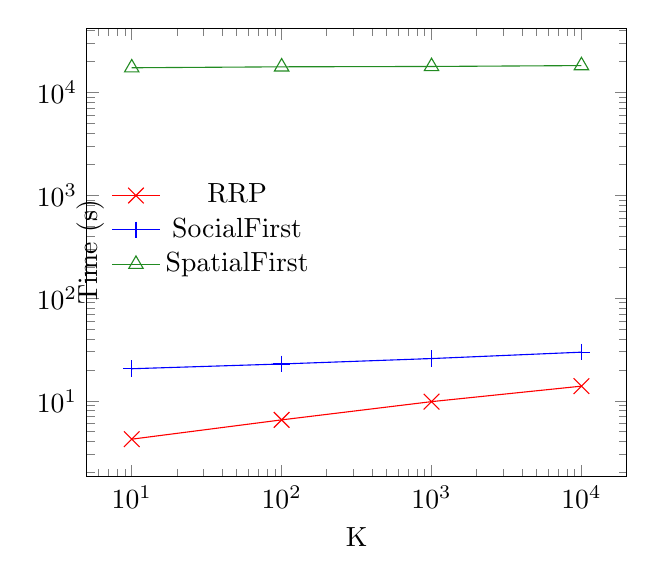
\begin{tikzpicture}[every plot/.append style={}]
	\begin{axis}[
	    xlabel={K},
	    ylabel={Time (s)},
	    xmode = log,
	    ymode = log,
	    legend style={at={(0.03,0.55)},anchor=west},
	    y label style={at={(axis description cs:0.05,.5)}},
		legend style={draw=none},
	    % legend pos=south east,
	    %xmajorgrids=true,
	    %ymajorgrids=true,
	    % xtick={0, 10, 20, 40, 80, 160, 320, 640, 1280},
	    % xticklabel style={rotate=90},
	    %grid style=dashed,
	    % axis line style = ultra thin
	]
	 
	\addplot[
	    color=red,
	    mark=x,
	    mark size=4pt
	    ]
	    coordinates {
	    (10, 4.23)(100, 6.52)(1000, 9.81)(10000, 13.88)
	    %(10, 4.23)(100, 6.52)(500, 9.33)(1000, 9.81)(5000, 13.88)(10000, 13.88)
	    };
	\addplot[
	    color=blue,
	    mark=+,
	    mark size=3pt
	    ]
	    coordinates {
	    (10, 20.5)(100, 22.81)(1000, 25.75)(10000, 29.71)
	    %(10, 20.5)(100, 22.81)(500, 23.04)(1000, 25.75)(5000, 26.61)(10000, 29.71)
	    };
	\addplot[
	    color=ForestGreen,
	    mark=triangle,
	    mark size=3pt
	    ]
	    coordinates {
	    (10, 17382.72)(100, 17755.99)(1000, 17896.76)(10000, 18254.65)
	    };
	    \legend{{\rrp}, SocialFirst, SpatialFirst}
	 
	\end{axis}
	\end{tikzpicture}
	\caption{Query time of different approaches by varying K}
	\label{fig:plot-01}
\end{figure}

{\rrp} is first compared with SocialFirst and SpatialFirst approaches introduced in section \ref{sec:preliminary}. Figure \ref{fig:plot-01} compares the time taken by {\rrp}, SpatialFirst and SocialFirst algorithms for the same source vertex and region. It may seem very intuitive at first that the SpatialFirst algorithm should totally beat others as it is pruning the graph by a huge extent initially using r-tree. To be exact from a graph of 629K nodes, we focused on 2,804 filtered nodes (by r-tree) only which is 0.44\% of the entire graph. Surprisingly, SpatialFirst is 3 orders of magnitude slower than the simple graph traversal SocialFirst algorithm and 4 orders of magnitude slower than {\rrp}. The reason for this massive difference is, A* with landmark is designed for solving single source and single destination problems. In our case A* with landmark function is invoked from the single given source vertex to every destination vertex in the region. Getting into some digits, say A* with landmark takes 3s (which is a very modest number on a real Yelp graph) for computing the shortest path for a given source and destination. Assume the given region R contains 2,000 venues. Therefore A* with landmark is invoked to each of them for a total of 2,000 times, which itself takes about 6,000s or 1.67 hours! Another way to visualize is, the algorithm (from source) is restarted for each of 2,000 destinations which causes it to lose by a huge margin with SocialFirst and {\rrp}.

That is where the SocialFirst algorithm shines. It totally takes a disconnected approach between spatial and social constraints like SpatialFirst, however it doesn't restart for obtaining the next shortest path. SpatialFirst aimlessly wanders the graph in the order of increasing distances from source and emits a result when it finds a vertex in the region. {\rrp} is the best of both the worlds, as it uses a heuristic to traverse the graph in a goal oriented manner towards the region like SpatialFirst and does not restart for obtaining the next shortest destination like SocialFirst. This is the main reason why it shines than the other approaches. And this can be clearly seen in Figure \ref{fig:plot-01}. As SpatialFirst is way out of the league, it is eliminated from the discussion from now on and SocialFirst and {\rrp} are focused. From the plot it is evident that as K increases, the time taken  by {\rrp} and SocialFirst also increases. Though it may be very unlikely that for a query to seek with K $>$ 20, {\rrp} still outperforms SocialFirst algorithm by at least 2 times even in the worst cases. To be specific, the region in the query has 2,804 spatial nodes and K was set as high as 10,000 nodes which is 100\% selectivity for that region and is testing the limits. As the final outcome is clear, the main focus would now be only on {\rrp}. As {\rrp} is made of Spatial Index and Social Index, {\rrp} was run multiple times with and without each index and to study how each of them perform.

\begin{figure*}[t]
	\begin{subfigure}[t]{0.33\textwidth}\centering
		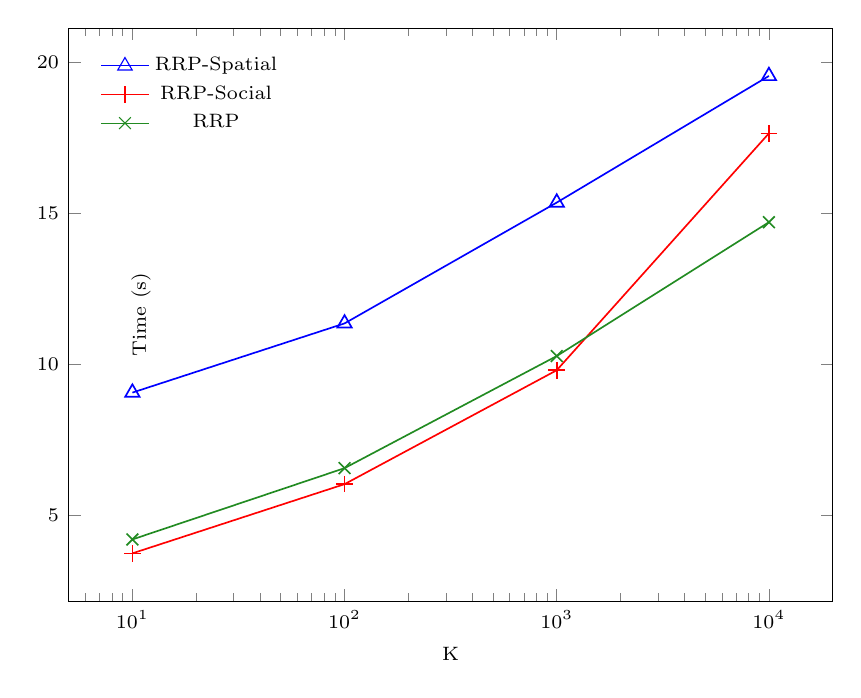
\begin{tikzpicture}[every plot/.append style={semithick}]
		\begin{axis}[
		every axis/.append style = {font = \scriptsize},
		scale only axis,
		width = 0.8\textwidth, height = 0.6\textwidth,
		xlabel={\scriptsize K},
		ylabel={\scriptsize Time (s)},
		y label style={at={(axis description cs:0.12,0.5)}},
		legend pos=north west,
		legend style={draw=none, fill=none,font=\scriptsize},
		xmode = log,
		%xmajorgrids=true,
		%ymajorgrids=true,
		%grid style=dashed,
		mark size=3pt
		]
			 
			%\addplot[
			%    color=blue,
			%    mark=x,
			%    ]
			%    coordinates {
			%    (10,73.8)(20,64.22)(40,64.06)(80,64.66)(160,69.06)(320,69.48)(640,64.44)(1280,64.44)
			%    };
			\addplot[
			    color=blue,
			    mark=triangle,
			    ]
			    coordinates {
			    (10, 9.07)(100, 11.36)(1000, 15.36)(10000, 19.55)
			    %(10, 9.07)(100, 11.36)(500, 13.59)(1000, 15.36)(5000, 19.45)(10000, 19.55)
			    };
			\addplot[
			    color=red,
			    mark=+,
			    ]
			    coordinates {
			    (10, 3.75)(100, 6.04)(1000, 9.81)(10000, 17.65)
			    %(10, 3.75)(100, 6.04)(500, 8.12)(1000, 9.81)(5000, 14.58)(10000, 17.65)
			    };
			\addplot[
			    color=ForestGreen,
			    mark=x,
			    ]
			    coordinates {
			    (10, 4.21)(100, 6.57)(1000, 10.28)(10000, 14.71)
			    %(10, 4.21)(100, 6.57)(500, 8.81)(1000, 10.28)(5000, 13.4)(10000, 14.71)
			    };
			%    \legend{SocialFirst, {\rrpspatial}, {\rrpsocial}, RRP}
			    \legend{{\rrpspatial}, {\rrpsocial}, {\rrp}}
			 
			\end{axis}
		\end{tikzpicture}
		% \caption{Runtime comparison between SocialFirst and types of {\rrp} algorithms for RZ = 10}
		\caption{RZ = 25}
		\label{fig:plot-02}
	\end{subfigure}
	\begin{subfigure}[t]{0.33\textwidth}
		\centering
		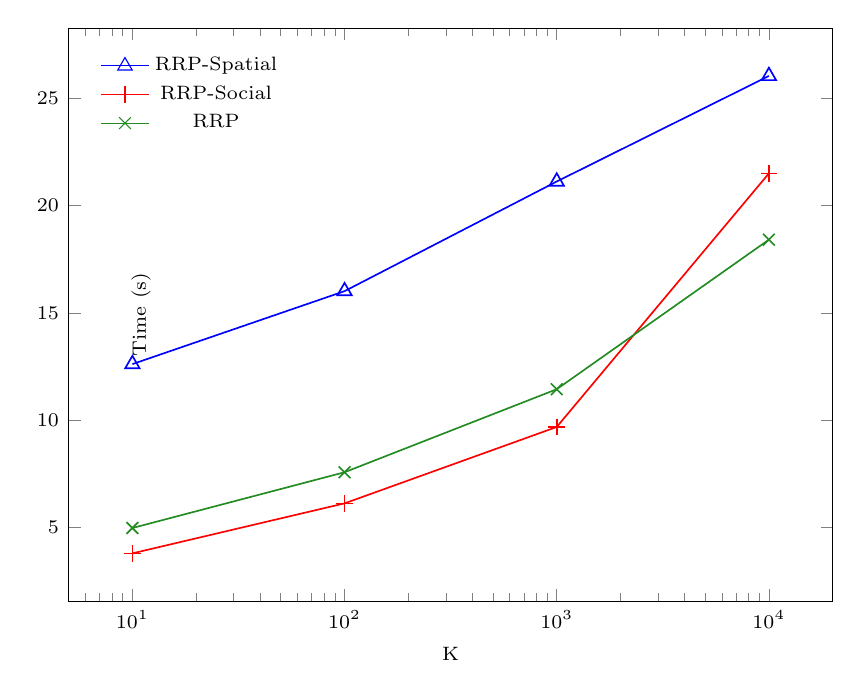
\begin{tikzpicture}[every plot/.append style={semithick}]
		\begin{axis}[
		every axis/.append style = {font = \scriptsize},
		scale only axis,
		width = 0.8\textwidth, height = 0.6\textwidth,
		xlabel={\scriptsize K},
		ylabel={\scriptsize Time (s)},
		y label style={at={(axis description cs:0.12,0.5)}},
		legend pos=north west,
		legend style={draw=none, fill=none,font=\scriptsize},
		xmode = log,
		%xmajorgrids=true,
		%ymajorgrids=true,
		%grid style=dashed,
		mark size=3pt
		]
			 
			% \addplot[
			%     color=blue,
			%     mark=x,
			%     ]
			%     coordinates {
			%     (10,32.23)(20,29.95)(40,24.9)(80,30.6)(160,24.82)(320,29.76)(640,24.97)(1280,25)
			%     };
			\addplot[
			    color=blue,
			    mark=triangle,
			    ]
			    coordinates {
			    (10, 12.61)(100, 16.01)(1000, 21.12)(10000, 26.04)
			    %(10, 12.61)(100, 16.01)(500, 19.3)(1000, 21.12)(5000, 26.01)(10000, 26.04)
			    };
			\addplot[
			    color=red,
			    mark=+,
			    ]
			    coordinates {
			    (10, 3.79)(100, 6.12)(1000, 9.68)(10000, 21.5)
				%(10, 3.79)(100, 6.12)(500, 8.13)(1000, 9.68)(5000, 19.23)(10000, 21.5)
			    };
			\addplot[
			    color=ForestGreen,
			    mark=x,
			    ]
			    coordinates {
			    (10, 4.97)(100, 7.57)(1000, 11.44)(10000, 18.41)
			    %(10, 4.97)(100, 7.57)(500, 9.86)(1000, 11.44)(5000, 15.81)(10000, 18.41)
			    };
			    % \legend{SocialFirst, {\rrpspatial}, {\rrpsocial}, {\rrp}}
			    \legend{{\rrpspatial}, {\rrpsocial}, {\rrp}}
			 
			\end{axis}
		\end{tikzpicture}
		% \caption{Runtime comparison between SocialFirst and types of {\rrp} algorithms for RZ = 1,000}
		\caption{RZ = 3125}
		\label{fig:plot-03}
	\end{subfigure}
	\begin{subfigure}[t]{0.33\textwidth}
		\centering
		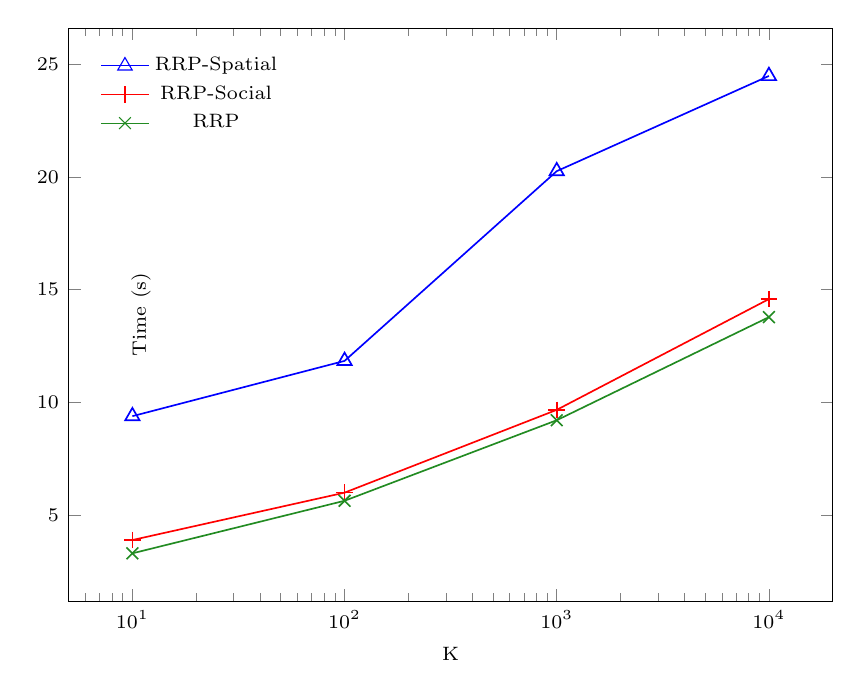
\begin{tikzpicture}[every plot/.append style={semithick}]
		\begin{axis}[
		every axis/.append style = {font = \scriptsize},
		scale only axis,
		width = 0.8\textwidth, height = 0.6\textwidth,
		xlabel={\scriptsize K},
		ylabel={\scriptsize Time (s)},
		y label style={at={(axis description cs:0.12,0.5)}},
		legend pos=north west,
		legend style={draw=none, fill=none,font=\scriptsize},
		xmode = log,
		%xmajorgrids=true,
		%ymajorgrids=true,
		%grid style=dashed,
		mark size=3pt
		]
			 
			\addplot[
			    color=blue,
			    mark=triangle,
			    ]
			    coordinates {
			    (10, 9.39)(100, 11.84)(1000, 20.25)(10000, 24.47)
			    %(10, 9.39)(100, 11.84)(500, 14.41)(1000, 20.25)(5000, 22.67)(10000, 24.47)
			    };
			\addplot[
			    color=red,
			    mark=+,
			    ]
			    coordinates {
			    (10, 3.9)(100, 6.0)(1000, 9.67)(10000, 14.58)
			    %(10, 3.9)(100, 6.0)(500, 8.07)(1000, 9.67)(5000, 14.56)(10000, 14.58)
			    };
			\addplot[
			    color=ForestGreen,
			    mark=x,
			    ]
			    coordinates {
			    (10, 3.31)(100, 5.64)(1000, 9.21)(10000, 13.78)
			    %(10, 3.31)(100, 5.64)(500, 7.69)(1000, 9.21)(5000, 13.46)(10000, 13.78)
			    };
			    \legend{{\rrpspatial}, {\rrpsocial}, {\rrp}}
			 
			\end{axis}
		\end{tikzpicture}
		\caption{RZ = 625, lower quality landmark}
		\label{fig:plot-09}
	\end{subfigure}
	\caption{Query time of {\rrp}, {\rrpsocial}, and {\rrpspatial} with different resolutions when varying K}
\end{figure*}

So the Figure \ref{fig:plot-02} breaks down the components of {\rrp} into {\rrpspatial}, {\rrpsocial} and Both (marked as {\rrp} in the plot's legend). {\rrpspatial} uses only the Spatial index while traversing the graph. As using only {\rrpspatial} index, a heuristic function cannot be built, modified Dijkstra's is used with one extra condition. In Dijkstra's, before adding any vertex to the priority queue, it is verified whether it can reach the given region R using the spatial index. So the sub graphs which cannot reach the region are pruned early using the index. Similarly, {\rrpsocial} uses only the social index for finding the K closest vertices to the source. For this, the algorithm is exactly like Algorithm \ref{alg3} except the condition on Line~\ref{alg:liesin} of Algorithm \ref{alg4} would always return \textbf{false}. This indirectly means spatial index is never used.

Though using either of the indices beat SocialFirst and of course SpatialFirst algorithms, it can be clearly seen that using {\rrpsocial} index outperforms others for smaller K in this case. To understand why it is so, revisit the heuristic algorithm of {\rrp}. The heuristic function uses the Social index with landmark(s). Combined with triangle inequality a lower bound on the distance between the source vertex and a destination vertex in the region is computed. Higher the lower bound, better is the pruning power of {\rrp}. As discussed the quality of landmark(s) plays an important role in the performance. So here using the spatial index only adds the overhead by querying that index, therefore the curve using both the indices slightly underperforms initially. But as K increases, the heuristic’s bound weakens as \textbf{v} in Figure \ref{fig:tri-ine} is no longer small compared to \textbf{u}. At the same time, spatial index helps {\rrp} to make better decisions whenever social index fails. The bottom line, using social index gives better results when: (1) Quality of the heuristic, indirectly landmarks, is very good; (2) Graph is very dense that most of the vertices can reach the region, making spatial index only an overhead.
%\begin{itemize}
%  \item Quality of the heuristic, indirectly landmarks, is very good
%  \item Graph is very dense that most of the vertices can reach the region, making spatial index only an overhead
%\end{itemize}

However, as the value of K increases, using both the indices certainly helps as un-necessary graph traversals are further reduced by spatial index. This is clearer in a later experiment when the quality of the landmark is not as good as this case. A very low resolution of 25 by 25 was used above. So how the runtimes change when we increase it by 125 times is studied next.

Just as expected as shown in Figure \ref{fig:plot-03}, the gap between {\rrp} and {\rrpsocial} indices further increases when resolution (RZ) is set to 3125. The function LIES\_IN which checks whether a vertex can reach a region using spatial index takes longer when size of the index entry increases for a given vertex. To totally confirm that this is the case, LIES\_IN was implemented in two more ways which were equivalent w.r.t. runtime but cash on \textit{tiny} advantages based on the size of R and size of spatial index. This is exactly the same parameter {\vra} in Table \ref{tab:default-param}. This is how each algorithm is implemented:
\begin{itemize}
  \item \textbf{Type 1}: In this axes transformation technique was used to check if a vertex reaches a region. The axes were transformed such that the southwest corner of the region in the query, is set as origin (0,0). Then for checking if a vertex reaches this region, spatial index entry for the vertex is queried. Then each block number, that the vertex can reach as per spatial index, is transformed into the new co-ordinate system. Then using this transformed 2D block number, a simple comparison of the block with all four corners of the region was used.
  \item \textbf{Type 2}: In this, region (R) in the query is enumerated to block numbers for as many levels as there in the spatial index. Then to check if a vertex reaches this region, each block number from the spatial index for the vertex, are probed with the enumerated region (R). This probing can be done in constant time if blocks reachable by a vertex are stored in a HashSet. This approach performs better than Type 1 if region is really small as the overhead of transforming into a new co-ordinate system is avoided.
  \item \textbf{Type 3}: In this also, region (R) in the query is enumerated to block numbers for all levels in the spatial index. Then a native set intersection function to find if there is match between blocks from R and blocks from a vertex was used. This sometimes shines as native programming implementations which are written in most optimized way especially in higher level languages like Python.
\end{itemize}

\begin{figure*}[t]
	\begin{subfigure}[t]{0.33\textwidth}
		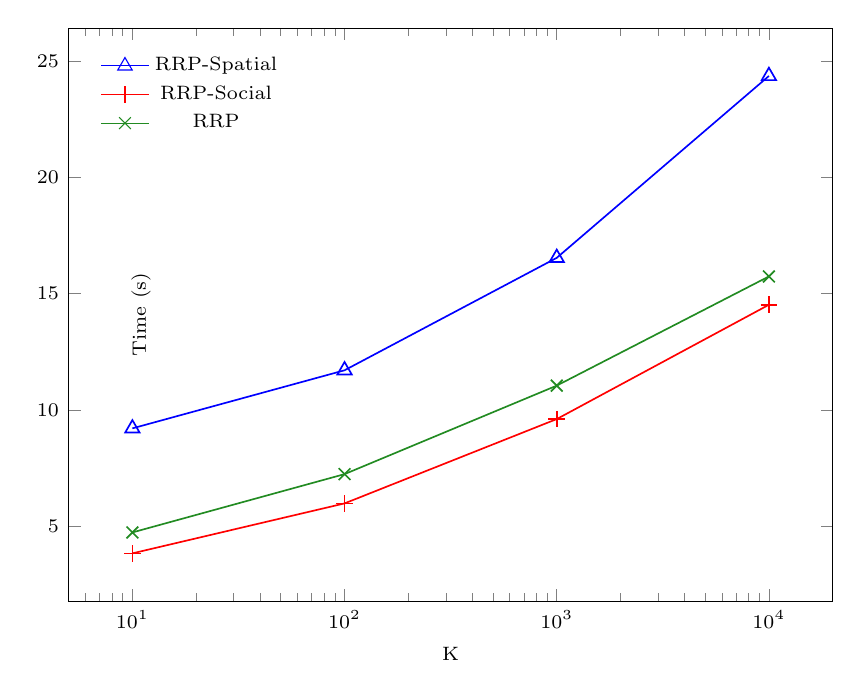
\begin{tikzpicture}[every plot/.append style={semithick}]
		\begin{axis}[
		every axis/.append style = {font = \scriptsize},
		scale only axis,
		width = 0.8\textwidth, height = 0.6\textwidth,
		xlabel={\scriptsize K},
		ylabel={\scriptsize Time (s)},
		y label style={at={(axis description cs:0.12,0.5)}},
		legend pos=north west,
		legend style={draw=none, fill=none,font=\scriptsize},
		xmode = log,
		%xmajorgrids=true,
		%ymajorgrids=true,
		%grid style=dashed,
		mark size=3pt
		]
			 
			% \addplot[
			%     color=blue,
			%     mark=x,
			%     ]
			%     coordinates {
			%     (10,25.67)(20,29.75)(40,25.14)(80,30.61)(160,24.84)(320,24.94)(640,24.95)(1280,24.94)
			%     };
			\addplot[
			    color=blue,
			    mark=triangle,
			    ]
			    coordinates {
			    (10, 9.2)(100, 11.7)(1000, 16.54)(10000, 24.37)
			    %(10, 9.2)(100, 11.7)(500, 13.79)(1000, 16.54)(5000, 19.49)(10000, 24.37)
			    };
			\addplot[
			    color=red,
			    mark=+,
			    ]
			    coordinates {
			    (10, 3.82)(100, 5.97)(1000, 9.6)(10000, 14.52)
				%(10, 3.82)(100, 5.97)(500, 8.02)(1000, 9.6)(5000, 14.5)(10000, 14.52)
			    };
			\addplot[
			    color=ForestGreen,
			    mark=x,
			    ]
			    coordinates {
			    (10, 4.72)(100, 7.23)(1000, 11.04)(10000, 15.74)
			    %(10, 4.72)(100, 7.23)(500, 9.41)(1000, 11.04)(5000, 15.48)(10000, 15.74)
			    };
			    % \legend{SocialFirst, {\rrpspatial}, {\rrpsocial}, {\rrp}}
			    \legend{{\rrpspatial}, {\rrpsocial}, {\rrp}}
			 
			\end{axis}
		\end{tikzpicture}
		\caption{{\vra} Type 1}
		\label{fig:plot-04}
	\end{subfigure}
	\begin{subfigure}[t]{0.33\textwidth}
		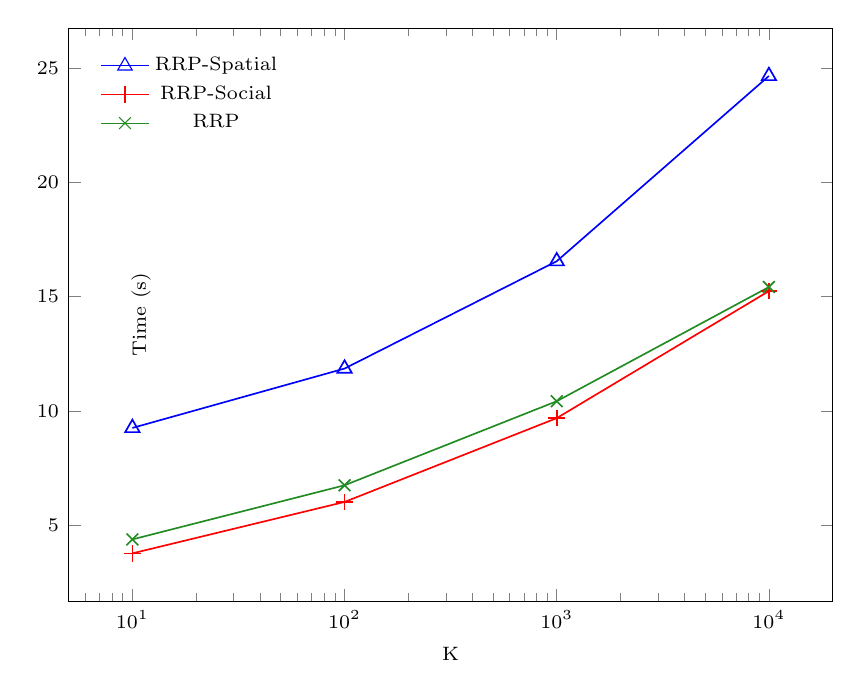
\begin{tikzpicture}[every plot/.append style={semithick}]
		\begin{axis}[
		every axis/.append style = {font = \scriptsize},
		scale only axis,
		width = 0.8\textwidth, height = 0.6\textwidth,
		xlabel={\scriptsize K},
		ylabel={\scriptsize Time (s)},
		y label style={at={(axis description cs:0.12,0.5)}},
		legend pos=north west,
		legend style={draw=none, fill=none,font=\scriptsize},
		xmode = log,
		%xmajorgrids=true,
		%ymajorgrids=true,
		%grid style=dashed,
		mark size=3pt
		]
			 
			% \addplot[
			%     color=blue,
			%     mark=x,
			%     ]
			%     coordinates {
			%     (10,26.11)(20,30.17)(40,25.41)(80,29.98)(160,25.37)(320,24.77)(640,25.03)(1280,24.82)
			%     };
			\addplot[
			    color=blue,
			    mark=triangle,
			    ]
			    coordinates {
			    (10, 9.25)(100, 11.85)(1000, 16.55)(10000, 24.66)
			    %(10, 9.25)(100, 11.85)(500, 13.84)(1000, 16.55)(5000, 19.6)(10000, 24.66)
			    };
			\addplot[
			    color=red,
			    mark=+,
			    ]
			    coordinates {
			    (10, 3.76)(100, 6.01)(1000, 9.68)(10000, 15.24)
				%(10, 3.76)(100, 6.01)(500, 8.14)(1000, 9.68)(5000, 14.71)(10000, 15.24)
			    };
			\addplot[
			    color=ForestGreen,
			    mark=x,
			    ]
			    coordinates {
			    (10, 4.37)(100, 6.74)(1000, 10.42)(10000, 15.42)
			    %(10, 4.37)(100, 6.74)(500, 8.87)(1000, 10.42)(5000, 14.79)(10000, 15.42)
			    };
			    % \legend{SocialFirst, {\rrpspatial}, {\rrpsocial}, {\rrp}}
			    \legend{{\rrpspatial}, {\rrpsocial}, {\rrp}}
			 
			\end{axis}
		\end{tikzpicture}
		% \caption{Runtime comparison between SocialFirst and types of {\rrp} algorithms using {\vra} Type 2 and RZ = 100}
		\caption{{\vra} Type 2}
		\label{fig:plot-05}
	\end{subfigure}
	\begin{subfigure}[t]{0.33\textwidth}
		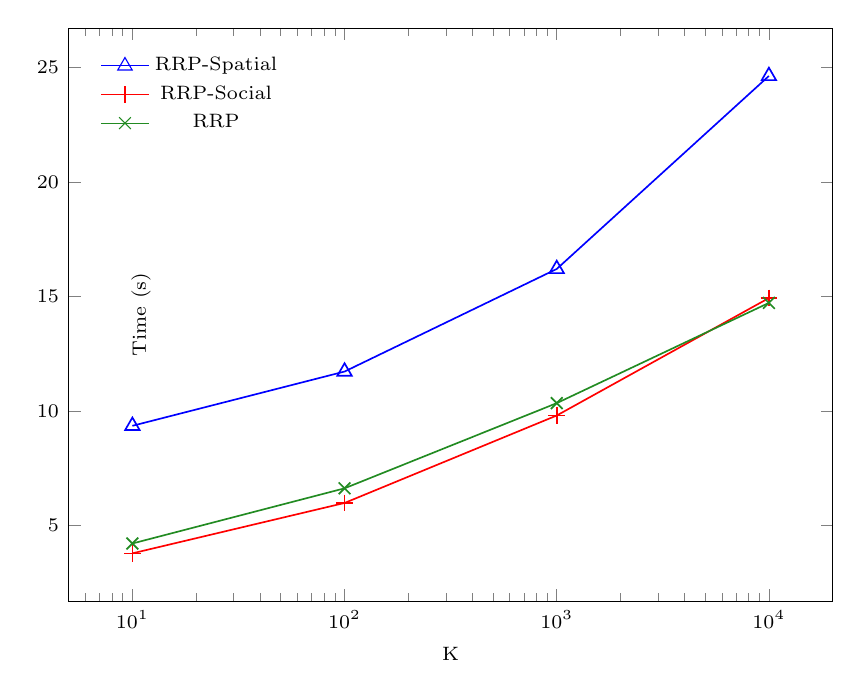
\begin{tikzpicture}[every plot/.append style={semithick}]
		\begin{axis}[
		every axis/.append style = {font = \scriptsize},
		scale only axis,
		width = 0.8\textwidth, height = 0.6\textwidth,
		xlabel={\scriptsize K},
		ylabel={\scriptsize Time (s)},
		y label style={at={(axis description cs:0.12,0.5)}},
		legend pos=north west,
		legend style={draw=none, fill=none,font=\scriptsize},
		xmode = log,
		%xmajorgrids=true,
		%ymajorgrids=true,
		%grid style=dashed,
		mark size=3pt
		]
			 
			% \addplot[
			%     color=blue,
			%     mark=x,
			%     ]
			%     coordinates {
			%     (10,25.14)(20,29.93)(40,25.51)(80,30.6)(160,24.84)(320,24.97)(640,25)(1280,25.09)
			%     };
			\addplot[
			    color=blue,
			    mark=triangle,
			    ]
			    coordinates {
			    (10, 9.36)(100, 11.73)(1000, 16.21)(10000, 24.64)
			    %(10, 9.36)(100, 11.73)(500, 14.41)(1000, 16.21)(5000, 19.95)(10000, 24.64)
			    };
			\addplot[
			    color=red,
			    mark=+,
			    ]
			    coordinates {
			    (10, 3.79)(100, 5.99)(1000, 9.81)(10000, 14.94)
				%(10, 3.79)(100, 5.99)(500, 8.1)(1000, 9.81)(5000, 14.66)(10000, 14.94)
			    };
			\addplot[
			    color=ForestGreen,
			    mark=x,
			    ]
			    coordinates {
			    (10, 4.22)(100, 6.63)(1000, 10.35)(10000, 14.73)
			    %(10, 4.22)(100, 6.63)(500, 8.77)(1000, 10.35)(5000, 14.75)(10000, 14.73)
			    };
			    % \legend{SocialFirst, {\rrpspatial}, {\rrpsocial}, {\rrp}}
			    \legend{{\rrpspatial}, {\rrpsocial}, {\rrp}}
			 
			\end{axis}
		\end{tikzpicture}
		% \caption{Runtime comparison between SocialFirst and types of {\rrp} algorithms using {\vra} Type 3 and RZ = 100}
		\caption{{\vra} Type 3}
		\label{fig:plot-06}
	\end{subfigure}
	\caption{Runtime comparison between the types of {\rrp} algorithms for RZ = 625 and various {\vra} Types}
\end{figure*}

That is how each of the three LIES\_IN algorithms are implemented. Figures \ref{fig:plot-04}, \ref{fig:plot-05}, \ref{fig:plot-06} clearly show that all perform the same way. However, if on mashing the plots together keeping the K constant, Algorithm of Type 3 outperforms in majority of the cases. This confirms the previous doubt that if the resolution is too high like 3125 by 3125 the overhead in LIES\_IN function overcomes the advantage gained by graph pruning in a dense graph. Now to figure out the sweet spot for right value of RZ, experiments comparing K VS Resolution VS Time for each variant of {\rrp} were studied. 

\begin{figure}[t]
	\begin{subfigure}[t]{0.23\textwidth}
		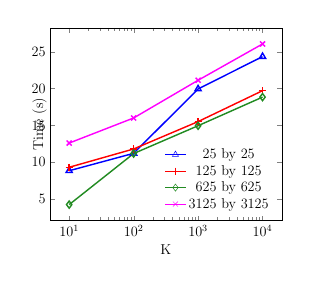
\begin{tikzpicture}[every plot/.append style={very thick}, scale=0.43]
			\begin{axis}[
			    xlabel={K},
			    ylabel={Time (s)},
			    legend pos=south east,
			    xmode = log,
			    %xmajorgrids=true,
			    %ymajorgrids=true,
			    %grid style=dashed,
			    mark size=3pt,
			    xtick=data,
			    % unit vector ratio=1 1 1,
			    % x=0.0015cm,
			    %xticklabels={10, 100, 500, 1000, 5000, 10000}
			    y label style={font=\large, at={(axis description cs:0.005,.5)}},
			    x label style={font=\large},
			    yticklabel style = {font=\large},
			    xticklabel style = {font=\large},
			    legend style={font=\large},
				legend style={draw=none},
			]
			 
			\addplot[
			    color=blue,
			    mark=triangle,
			    ]
			    coordinates {
			    (10, 8.86)(100, 11.22)(1000, 19.94)(10000, 24.33)
			    % (10, 8.86)(100, 11.22)(500, 18.45)(1000, 19.94)(5000, 24.31)(10000, 24.33)
			    %(1, 8.86)(2, 11.22)(3, 18.45)(4, 19.94)(5, 24.31)(6, 24.33)
			    };
			% \addplot[
			%     color=Maroon,
			%     mark=square,
			%     ]
			%     coordinates {
			%     % (10, 4.14)(100, 11.64)(500, 13.52)(1000, 15.1)(5000, 19.33)(10000, 19.31)
			%     (1, 4.14)(2, 11.64)(3, 18.52)(4, 15.1)(5, 19.33)(6, 19.31)
			%     };
			\addplot[
			    color=red,
			    mark=+,
			    ]
			    coordinates {
			    (10, 9.33)(100, 11.81)(1000, 15.52)(10000, 19.71)
				% (10, 9.33)(100, 11.81)(500, 13.82)(1000, 15.52)(5000, 19.66)(10000, 19.71)
				%(1, 9.33)(2, 11.81)(3, 13.82)(4, 15.52)(5, 19.66)(6, 19.71)
			    };
			\addplot[
			    color=ForestGreen,
			    mark=diamond,
			    ]
			    coordinates {
			    (10, 4.27)(100, 11.19)(1000, 14.96)(10000, 18.84)
			    % (10, 4.27)(100, 11.19)(500, 13.4)(1000, 14.96)(5000, 19.02)(10000, 18.84)
			    %(1, 4.27)(2, 11.19)(3, 13.4)(4, 14.96)(5, 19.02)(6, 18.84)
			    };
			\addplot[
			    color=Magenta,
			    mark=x,
			    ]
			    coordinates {
			    (10, 12.61)(100, 16.01)(1000, 21.12)(10000, 26.04)
			    % (10, 12.61)(100, 16.01)(500, 19.3)(1000, 21.12)(5000, 26.01)(10000, 26.04)
			    %(1, 12.61)(2, 16.01)(3, 19.3)(4, 21.12)(5, 26.01)(6, 26.04)
			    };
			    % \legend{5 by 5,25 by 25,125 by 125,625 by 625,3125 by 3125}
			    \legend{25 by 25,125 by 125,625 by 625,3125 by 3125}
			 
			\end{axis}
		\end{tikzpicture}
		\caption{{\rrpspatial}}
		\label{fig:plot-07}
	\end{subfigure}
	\begin{subfigure}[t]{0.23\textwidth}
		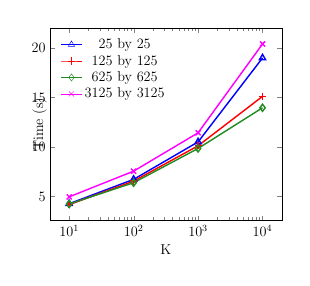
\begin{tikzpicture}[every plot/.append style={very thick}, scale=0.43]
			\begin{axis}[
			    xlabel={K},
			    ylabel={Time (s)},
			    legend pos=north west,
			    xmode = log,
			    %xmajorgrids=true,
			    %ymajorgrids=true,
			    %grid style=dashed,
			    mark size=3pt,
			    xtick=data,
			    %xticklabels={10, 100, 500, 1000, 5000, 10000}
			    y label style={font=\large, at={(axis description cs:0.005,.5)}},
			    x label style={font=\large},
			    yticklabel style = {font=\large},
			    xticklabel style = {font=\large},
			    legend style={font=\large},
				legend style={draw=none},
			]
			 
			\addplot[
			    color=blue,
			    mark=triangle,
			    ]
			    coordinates {
			    (10, 4.28)(100, 6.74)(1000, 10.52)(10000, 19.0)
			    % (10, 4.28)(100, 6.74)(500, 8.92)(1000, 10.52)(5000, 16.09)(10000, 19.0)
			    %(1, 4.28)(2, 6.74)(3, 8.92)(4, 10.52)(5, 16.09)(6, 19.0)
			    };
			% \addplot[
			%     color=Maroon,
			%     mark=square,
			%     ]
			%     coordinates {
			%     % (10, 4.26)(100, 6.67)(500, 8.83)(1000, 10.23)(5000, 14.64)(10000, 14.62)
			%     (1, 4.26)(2, 6.67)(3, 8.83)(4, 10.23)(5, 14.64)(6, 14.62)
			%     };
			\addplot[
			    color=red,
			    mark=+,
			    ]
			    coordinates {
			    (10, 4.19)(100, 6.56)(1000, 10.13)(10000, 15.12)
				% (10, 4.19)(100, 6.56)(500, 8.7)(1000, 10.13)(5000, 14.39)(10000, 15.12)
				%(1, 4.19)(2, 6.56)(3, 8.7)(4, 10.13)(5, 14.39)(6, 15.12)
			    };
			\addplot[
			    color=ForestGreen,
			    mark=diamond,
			    ]
			    coordinates {
			    (10, 4.25)(100, 6.4)(1000, 9.86)(10000, 13.97)
			    % (10, 4.25)(100, 6.4)(500, 8.4)(1000, 9.86)(5000, 13.92)(10000, 13.97)
			    %(1, 4.25)(2, 6.4)(3, 8.4)(4, 9.86)(5, 13.92)(6, 13.97)
			    };
			\addplot[
			    color=Magenta,
			    mark=x,
			    ]
			    coordinates {
			    (10, 4.97)(100, 7.57)(1000, 11.44)(10000, 20.41)
			    % (10, 4.97)(100, 7.57)(500, 9.86)(1000, 11.44)(5000, 16.81)(10000, 20.41)
			    %(1, 4.97)(2, 7.57)(3, 9.86)(4, 11.44)(5, 16.81)(6, 20.41)
			    };
			    % \legend{5 by 5,25 by 25,125 by 125,625 by 625,3125 by 3125}
			    \legend{25 by 25,125 by 125,625 by 625,3125 by 3125}
			 
			\end{axis}
		\end{tikzpicture}
		\caption{{\rrp}}
		\label{fig:plot-08}
	\end{subfigure}
	\caption{Query time of {\rrpspatial} and {\rrp} with different resolutions}
	%\caption{Runtime comparison between Resolution and K for different types of {\rrp} algorithms}
\end{figure}

From Figure \ref{fig:plot-07} it is evident that as resolution increases for a fixed K and for {\rrpspatial}, performance degrades for very high resolutions due to the overhead by LIES\_IN function. For very low resolutions, as each block is almost the size of Texas, even if a user checks-in at one restaurant there, he/she is considered reachable to that block. So it returns that most vertices can reach R, making it less useful to use a spatial index. The sweet spot so is in between the both extremes, which is 625 in this case. Similar conclusions can be made in next case Figure \ref{fig:plot-08} where both indices were used. But social index lessens the loss brought by spatial index overhead and therefore extreme high resolutions also perform at par with lesser resolutions for smaller K. For larger K even quality of heuristic goes down, so the gap widens.

So after these experiments, it can be concluded that when the graph is really dense using the social index with a high quality landmark is sufficient. Things change when the quality of landmark(s) is not as good. For the next query, the region is even more densely connected and the source vertex is the same, however a lower quality landmark was used. This region has 21,239 spatial nodes which is almost 10 times the count of the previous one.

Figure \ref{fig:plot-09} proves why just having a social index wont help like before. For this region, purposefully a lower quality landmark was chosen. In such cases spatial index prunes majority of the graph as a good resolution of 625 by 625 found earlier was used. Though social index equally performed social+spatial index initially, it lost soon as the landmark quality further degraded for higher K for the same reason explained before. The correctness is never compromised, it is only that {\rrp} tends to Dijkstra's search if landmark quality is not good. Now that when to use each type of index is understood, how each of the algorithms perform with change in region size is studied next.

\begin{figure}[t]
	\begin{subfigure}[t]{0.23\textwidth}
		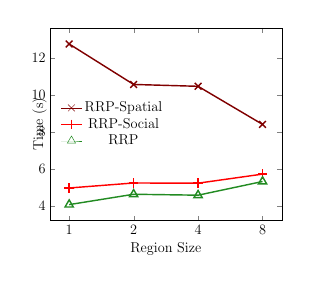
\begin{tikzpicture}[every plot/.append style={very thick}, scale=0.43]
			\begin{axis}[
			    xlabel={Region Size},
			    ylabel={Time (s)},
			    % legend pos=south west,
			    legend style={at={(0.03,0.5)},anchor=west},
			    % legend style={at={(0,-0.1)},anchor=north},
			    %xmajorgrids=true,
			    %ymajorgrids=true,
			    %grid style=dashed,
			    mark size=4pt,
			    xtick=data,
			    xticklabels={1, 2, 4, 8},
			    y label style={font=\large, at={(axis description cs:0.005,.5)}},
			    x label style={font=\large},
			    yticklabel style = {font=\large},
			    xticklabel style = {font=\large},
			    legend style={font=\large},
				legend style={draw=none},
			]
			 
			% \addplot[
			%     color=blue,
			%     mark=x,
			%     ]
			%     coordinates {
			%     (1, 25.81058407)(2, 30.50130916)(4, 31.07799816)(8, 32.95914412)
			%     };
			\addplot[
			    color=Maroon,
			    mark=x,
			    ]
			    coordinates {
			    (1, 12.77)(2, 10.58)(3, 10.48)(4, 8.42)
			    };
			\addplot[
			    color=red,
			    mark=+,
			    ]
			    coordinates {
			    (1, 4.98)(2, 5.25)(3, 5.24)(4, 5.73)
			    };
			\addplot[
			    color=ForestGreen,
			    mark=triangle,
			    ]
			    coordinates {
			    (1, 4.08)(2, 4.64)(3, 4.59)(4, 5.33)
			    };
			    % \legend{SocialFirst, {\rrpspatial}, {\rrpsocial}, {\rrp}}
			    \legend{{\rrpspatial}, {\rrpsocial}, {\rrp}}
			 
			\end{axis}
		\end{tikzpicture}
		% \caption{Runtime comparison between SocialFirst and types of {\rrp} algorithms for changes in region size for a source vertex S1}
		\caption{Source = S1}
		\label{fig:plot-10}
	\end{subfigure}
	\begin{subfigure}[t]{0.23\textwidth}
		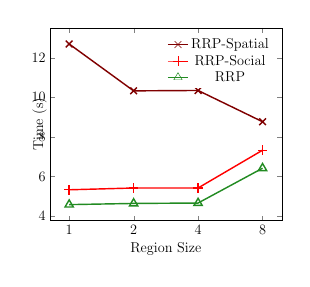
\begin{tikzpicture}[every plot/.append style={very thick}, scale=0.43]
			\begin{axis}[
			    xlabel={Region Size},
			    ylabel={Time (s)},
			    legend pos=north east,
			    %xmajorgrids=true,
			    %ymajorgrids=true,
			    %grid style=dashed,
			    mark size=4pt,
			    xtick=data,
			    xticklabels={1, 2, 4, 8},
			    y label style={font=\large, at={(axis description cs:0.005,.5)}},
			    x label style={font=\large},
			    yticklabel style = {font=\large},
			    xticklabel style = {font=\large},
			    legend style={font=\large},
			    x label style={font=\large},
				legend style={draw=none},
			]
			 
			% \addplot[
			%     color=blue,
			%     mark=x,
			%     ]
			%     coordinates {
			%     (1, 26.25)(2, 30.53)(4, 30.52)(8, 32.17)
			%     };
			\addplot[
			    color=Maroon,
			    mark=x,
			    ]
			    coordinates {
			    (1, 12.7)(2, 10.33)(3, 10.35)(4, 8.77)
			    };
			\addplot[
			    color=red,
			    mark=+,
			    ]
			    coordinates {
			    (1, 5.33)(2, 5.42)(3, 5.42)(4, 7.33)
			    };
			\addplot[
			    color=ForestGreen,
			    mark=triangle,
			    ]
			    coordinates {
			    (1, 4.58)(2, 4.64)(3, 4.66)(4, 6.42)
			    };
			    % \legend{SocialFirst, {\rrpspatial}, {\rrpsocial}, {\rrp}}
			    \legend{{\rrpspatial}, {\rrpsocial}, {\rrp}}
			 
			\end{axis}
		\end{tikzpicture}
		% \caption{Runtime comparison between SocialFirst and types of {\rrp} algorithms for changes in region size for a source vertex S2}
		\caption{Source = S2}
		\label{fig:plot-11}
	\end{subfigure}
	\caption{Query time }
	%\caption{Runtime comparison between the types of {\rrp} algorithms VS region size for different source vertices}
	\label{fig:plot1011}
\end{figure}

Figure \ref{fig:plot-10} shows how in every algorithm the time taken linearly increase w.r.t. the size of the region. In Figure \ref{fig:plot1011}, in both the cases users near the source vertex have many check-ins in the given regions and so the spatial index performs worse initially due to its overhead but gradually performs better. The gap further reduces when we a user whose social neighbors do not have many check-ins in the query regions was chosen. Due to this algorithm has to traverse the social graph further down to find the result as shown in Figure \ref{fig:plot-11}.


\section{Conclusion} \label{sec:conclusion}
{\rrp} combines social and spatial searches which work on any GeoSocial graph. Different tunable parameters give an extra layer of flexibility to such a generic solution. Thorough experiments not only prove this point by outperforming existing approaches by at least 3 times even in extreme cases but also show how to set each of the tunable arguments. Extensions to {\rrp} can include a persistent way to store the index and also a distributed {\rrp} algorithm.


\bibliography{reference}
\bibliographystyle{plain}


\begin{center}\rule{0.5\linewidth}{\linethickness}\end{center}

\end{document}